% I seguenti commenti speciali impostano:
% 1. 
% 2. PDFLaTeX come motore di composizione;
% 3. tesi.tex come documento principale;
% 4. il controllo ortografico italiano per l'editor.

% !TEX encoding = UTF-8
% !TEX TS-program = pdflatex
% !TEX root = tesi.tex
% !TEX spellcheck = it-IT

% PDF/A filecontents
\RequirePackage{filecontents}
\begin{filecontents*}{\jobname.xmpdata}
  \Title{Document’s title}
  \Author{Author’s name}
  \Language{it-IT}
  \Subject{The abstract, or short description.}
  \Keywords{keyword1\sep keyword2\sep keyword3}
\end{filecontents*}

\documentclass[10pt,                    % corpo del font principale
               a4paper,                 % carta A4
               twoside,                 % impagina per fronte-retro
               openright,               % inizio capitoli a destra
               english,                 
               italian,                 
               ]{book}    

%**************************************************************
% Importazione package
%************************************************************** 

\PassOptionsToPackage{dvipsnames}{xcolor} % colori PDF/A

\usepackage{colorprofiles}

\usepackage[a-2b,mathxmp]{pdfx}[2018/12/22]
                                        % configurazione PDF/A
                                        % validare in https://www.pdf-online.com/osa/validate.aspx

%\usepackage{amsmath,amssymb,amsthm}    % matematica

\usepackage[T1]{fontenc}                % codifica dei font:
                                        % NOTA BENE! richiede una distribuzione *completa* di LaTeX

\usepackage[utf8]{inputenc}             % codifica di input; anche [latin1] va bene
                                        % NOTA BENE! va accordata con le preferenze dell'editor

\usepackage[english, italian]{babel}    % per scrivere in italiano e in inglese;
                                        % l'ultima lingua (l'italiano) risulta predefinita

\usepackage{bookmark}                   % segnalibri

\usepackage{caption}                    % didascalie

\usepackage{chngpage,calc}              % centra il frontespizio

\usepackage{csquotes}                   % gestisce automaticamente i caratteri (")

\usepackage{emptypage}                  % pagine vuote senza testatina e piede di pagina

\usepackage{epigraph}			% per epigrafi

\usepackage{eurosym}                    % simbolo dell'euro

%\usepackage{indentfirst}               % rientra il primo paragrafo di ogni sezione

\usepackage{graphicx}                   % immagini

\usepackage{hyperref}                   % collegamenti ipertestuali

\usepackage[binding=5mm]{layaureo}      % margini ottimizzati per l'A4; rilegatura di 5 mm

\usepackage{listings}                   % codici

\usepackage{microtype}                  % microtipografia

\usepackage{mparhack,fixltx2e,relsize}  % finezze tipografiche

\usepackage{nameref}                    % visualizza nome dei riferimenti                                      
\usepackage[font=small]{quoting}        % citazioni

\usepackage{subfig}                     % sottofigure, sottotabelle

\usepackage[italian]{varioref}          % riferimenti completi della pagina

\usepackage{booktabs}                   % tabelle                                       
\usepackage{tabularx}                   % tabelle di larghezza prefissata                                    
\usepackage{longtable}                  % tabelle su più pagine                                        
\usepackage{ltxtable}                   % tabelle su più pagine e adattabili in larghezza

\usepackage[toc, acronym]{glossaries}   % glossario
                                        % per includerlo nel documento bisogna:
                                        % 1. compilare una prima volta tesi.tex;
                                        % 2. eseguire: makeindex -s tesi.ist -t tesi.glg -o tesi.gls tesi.glo
                                        % 3. eseguire: makeindex -s tesi.ist -t tesi.alg -o tesi.acr tesi.acn
                                        % 4. compilare due volte tesi.tex.

\usepackage[backend=biber,style=verbose-ibid,hyperref,backref]{biblatex}
                                        % eccellente pacchetto per la bibliografia; 
                                        % produce uno stile di citazione autore-anno; 
                                        % lo stile "numeric-comp" produce riferimenti numerici
                                        % per includerlo nel documento bisogna:
                                        % 1. compilare una prima volta tesi.tex;
                                        % 2. eseguire: biber tesi
                                        % 3. compilare ancora tesi.tex.

%**************************************************************
% file contenente le impostazioni della tesi
%**************************************************************

%**************************************************************
% Frontespizio
%**************************************************************

% Autore
\newcommand{\myName}{Edoardo Caregnato}                                    
\newcommand{\myTitle}{Containerizzazione ed orchestrazione di applicativi .NET tramite utilizzo di Docker \& Docker Compose}

% Tipo di tesi                   
\newcommand{\myDegree}{Tesi di laurea triennale}

% Università             
\newcommand{\myUni}{Università degli Studi di Padova}

% Facoltà       
\newcommand{\myFaculty}{Corso di Laurea in Informatica}

% Dipartimento
\newcommand{\myDepartment}{Dipartimento di Matematica "Tullio Levi-Civita"}

% Titolo del relatore
\newcommand{\profTitle}{Prof. }

% Relatore
\newcommand{\myProf}{Massimo Marchiori}

% Luogo
\newcommand{\myLocation}{Padova}

% Anno accademico
\newcommand{\myAA}{2021-2022}

% Data discussione
\newcommand{\myTime}{Dicembre 2022}


%**************************************************************
% Impostazioni di impaginazione
% see: http://wwwcdf.pd.infn.it/AppuntiLinux/a2547.htm
%**************************************************************

\setlength{\parindent}{14pt}   % larghezza rientro della prima riga
\setlength{\parskip}{0pt}   % distanza tra i paragrafi


%**************************************************************
% Impostazioni di biblatex
%**************************************************************
\bibliography{bibliografia} % database di biblatex 

\defbibheading{bibliography} {
    \cleardoublepage
    \phantomsection 
    \addcontentsline{toc}{chapter}{\bibname}
    \chapter*{\bibname\markboth{\bibname}{\bibname}}
}

\setlength\bibitemsep{1.5\itemsep} % spazio tra entry

\DeclareBibliographyCategory{opere}
\DeclareBibliographyCategory{web}

\addtocategory{opere}{womak:lean-thinking}
\addtocategory{web}{site:agile-manifesto}

\defbibheading{opere}{\section*{Riferimenti bibliografici}}
\defbibheading{web}{\section*{Siti Web consultati}}


%**************************************************************
% Impostazioni di caption
%**************************************************************
\captionsetup{
    tableposition=top,
    figureposition=bottom,
    font=small,
    format=hang,
    labelfont=bf
}

%**************************************************************
% Impostazioni di glossaries
%**************************************************************

%**************************************************************
% Acronimi
%**************************************************************
\renewcommand{\acronymname}{Acronimi e abbreviazioni}

\newacronym[description={\glslink{apig}{Application Program Interface}}]
    {api}{API}{Application Program Interface}

\newacronym[description={\glslink{umlg}{Unified Modeling Language}}]
    {uml}{UML}{Unified Modeling Language}

%**************************************************************
% Glossario
%**************************************************************
%\renewcommand{\glossaryname}{Glossario}

\newglossaryentry{apig}
{
    name=\glslink{api}{API},
    text=Application Program Interface,
    sort=api,
    description={in informatica con il termine \emph{Application Programming Interface API} (ing. interfaccia di programmazione di un'applicazione) si indica ogni insieme di procedure disponibili al programmatore, di solito raggruppate a formare un set di strumenti specifici per l'espletamento di un determinato compito all'interno di un certo programma. La finalità è ottenere un'astrazione, di solito tra l'hardware e il programmatore o tra software a basso e quello ad alto livello semplificando così il lavoro di programmazione}
}

\newglossaryentry{umlg}
{
    name=\glslink{uml}{UML},
    text=UML,
    sort=uml,
    description={in ingegneria del software \emph{UML, Unified Modeling Language} (ing. linguaggio di modellazione unificato) è un linguaggio di modellazione e specifica basato sul paradigma object-oriented. L'\emph{UML} svolge un'importantissima funzione di ``lingua franca'' nella comunità della progettazione e programmazione a oggetti. Gran parte della letteratura di settore usa tale linguaggio per descrivere soluzioni analitiche e progettuali in modo sintetico e comprensibile a un vasto pubblico}
}

\newglossaryentry{API}
{
    name=\glslink{api}{API},
    text=API,
    sort=api, 
    description={in ingegneria del software \emph{UML, Unified Modeling Language} (ing. linguaggio di modellazione unificato) è un linguaggio di modellazione e specifica basato sul paradigma object-oriented. L'\emph{UML} svolge un'importantissima funzione di ``lingua franca'' nella comunità della progettazione e programmazione a oggetti. Gran parte della letteratura di settore usa tale linguaggio per descrivere soluzioni analitiche e progettuali in modo sintetico e comprensibile a un vasto pubblico}
}

\newglossaryentry{Container}
{
    name=\glslink{container}{CONTAINER},
    text=Container,
    sort=container, 
    description={in ingegneria del software \emph{UML, Unified Modeling Language} (ing. linguaggio di modellazione unificato) è un linguaggio di modellazione e specifica basato sul paradigma object-oriented. L'\emph{UML} svolge un'importantissima funzione di ``lingua franca'' nella comunità della progettazione e programmazione a oggetti. Gran parte della letteratura di settore usa tale linguaggio per descrivere soluzioni analitiche e progettuali in modo sintetico e comprensibile a un vasto pubblico}
}

\newglossaryentry{hardware}
{
    name=\glslink{hardware}{HARDWARE},
    text=hardware,
    sort=hardware, 
    description={in ingegneria del software \emph{UML, Unified Modeling Language} (ing. linguaggio di modellazione unificato) è un linguaggio di modellazione e specifica basato sul paradigma object-oriented. L'\emph{UML} svolge un'importantissima funzione di ``lingua franca'' nella comunità della progettazione e programmazione a oggetti. Gran parte della letteratura di settore usa tale linguaggio per descrivere soluzioni analitiche e progettuali in modo sintetico e comprensibile a un vasto pubblico}
}

\newglossaryentry{software}
{
    name=\glslink{software}{SOFTWARE},
    text=software,
    sort=software, 
    description={in ingegneria del software \emph{UML, Unified Modeling Language} (ing. linguaggio di modellazione unificato) è un linguaggio di modellazione e specifica basato sul paradigma object-oriented. L'\emph{UML} svolge un'importantissima funzione di ``lingua franca'' nella comunità della progettazione e programmazione a oggetti. Gran parte della letteratura di settore usa tale linguaggio per descrivere soluzioni analitiche e progettuali in modo sintetico e comprensibile a un vasto pubblico}
}

\newglossaryentry{Virtual Machine}
{
    name=\glslink{virtual machine}{VIRTUAL MACHINE},
    text=Virtual Machine,
    sort=virtual machine, 
    description={in ingegneria del software \emph{UML, Unified Modeling Language} (ing. linguaggio di modellazione unificato) è un linguaggio di modellazione e specifica basato sul paradigma object-oriented. L'\emph{UML} svolge un'importantissima funzione di ``lingua franca'' nella comunità della progettazione e programmazione a oggetti. Gran parte della letteratura di settore usa tale linguaggio per descrivere soluzioni analitiche e progettuali in modo sintetico e comprensibile a un vasto pubblico}
}

\newglossaryentry{Docker}
{
    name=\glslink{docker}{DOCKER},
    text=Docker,
    sort=docker, 
    description={in ingegneria del software \emph{UML, Unified Modeling Language} (ing. linguaggio di modellazione unificato) è un linguaggio di modellazione e specifica basato sul paradigma object-oriented. L'\emph{UML} svolge un'importantissima funzione di ``lingua franca'' nella comunità della progettazione e programmazione a oggetti. Gran parte della letteratura di settore usa tale linguaggio per descrivere soluzioni analitiche e progettuali in modo sintetico e comprensibile a un vasto pubblico}
}

\newglossaryentry{HDA}
{
    name=\glslink{hda}{HDA},
    text=HDA,
    sort=hda, 
    description={in ingegneria del software \emph{UML, Unified Modeling Language} (ing. linguaggio di modellazione unificato) è un linguaggio di modellazione e specifica basato sul paradigma object-oriented. L'\emph{UML} svolge un'importantissima funzione di ``lingua franca'' nella comunità della progettazione e programmazione a oggetti. Gran parte della letteratura di settore usa tale linguaggio per descrivere soluzioni analitiche e progettuali in modo sintetico e comprensibile a un vasto pubblico}
}

\newglossaryentry{Docker Compose}
{
    name=\glslink{docker compose}{DOCKER COMPOSE},
    text=Docker-Compose,
    sort=docker compose, 
    description={in ingegneria del software \emph{UML, Unified Modeling Language} (ing. linguaggio di modellazione unificato) è un linguaggio di modellazione e specifica basato sul paradigma object-oriented. L'\emph{UML} svolge un'importantissima funzione di ``lingua franca'' nella comunità della progettazione e programmazione a oggetti. Gran parte della letteratura di settore usa tale linguaggio per descrivere soluzioni analitiche e progettuali in modo sintetico e comprensibile a un vasto pubblico}
}

\newglossaryentry{CX Studio}
{
    name=\glslink{cx studio}{CX STUDIO},
    text=CX studio,
    sort=cx studio, 
    description={in ingegneria del software \emph{UML, Unified Modeling Language} (ing. linguaggio di modellazione unificato) è un linguaggio di modellazione e specifica basato sul paradigma object-oriented. L'\emph{UML} svolge un'importantissima funzione di ``lingua franca'' nella comunità della progettazione e programmazione a oggetti. Gran parte della letteratura di settore usa tale linguaggio per descrivere soluzioni analitiche e progettuali in modo sintetico e comprensibile a un vasto pubblico}
}

\newglossaryentry{client}
{
    name=\glslink{client}{CLIENT},
    text=client,
    sort=client, 
    description={in ingegneria del software \emph{UML, Unified Modeling Language} (ing. linguaggio di modellazione unificato) è un linguaggio di modellazione e specifica basato sul paradigma object-oriented. L'\emph{UML} svolge un'importantissima funzione di ``lingua franca'' nella comunità della progettazione e programmazione a oggetti. Gran parte della letteratura di settore usa tale linguaggio per descrivere soluzioni analitiche e progettuali in modo sintetico e comprensibile a un vasto pubblico}
}

\newglossaryentry{sistemi operativi}
{
    name=\glslink{sistemi operativi}{SISTEMI OPERATIVI},
    text=sistemi operativi,
    sort=sistemi operativi, 
    description={in ingegneria del software \emph{UML, Unified Modeling Language} (ing. linguaggio di modellazione unificato) è un linguaggio di modellazione e specifica basato sul paradigma object-oriented. L'\emph{UML} svolge un'importantissima funzione di ``lingua franca'' nella comunità della progettazione e programmazione a oggetti. Gran parte della letteratura di settore usa tale linguaggio per descrivere soluzioni analitiche e progettuali in modo sintetico e comprensibile a un vasto pubblico}
}

\newglossaryentry{Hyper-V}
{
    name=\glslink{hyper-v}{HYPER-V},
    text=Hyper-V,
    sort=hyper-v, 
    description={in ingegneria del software \emph{UML, Unified Modeling Language} (ing. linguaggio di modellazione unificato) è un linguaggio di modellazione e specifica basato sul paradigma object-oriented. L'\emph{UML} svolge un'importantissima funzione di ``lingua franca'' nella comunità della progettazione e programmazione a oggetti. Gran parte della letteratura di settore usa tale linguaggio per descrivere soluzioni analitiche e progettuali in modo sintetico e comprensibile a un vasto pubblico}
}

\newglossaryentry{Xen}
{
    name=\glslink{xen}{XEN},
    text=Xen,
    sort=xen, 
    description={in ingegneria del software \emph{UML, Unified Modeling Language} (ing. linguaggio di modellazione unificato) è un linguaggio di modellazione e specifica basato sul paradigma object-oriented. L'\emph{UML} svolge un'importantissima funzione di ``lingua franca'' nella comunità della progettazione e programmazione a oggetti. Gran parte della letteratura di settore usa tale linguaggio per descrivere soluzioni analitiche e progettuali in modo sintetico e comprensibile a un vasto pubblico}
}

\newglossaryentry{host}
{
    name=\glslink{host}{HOST},
    text=host,
    sort=host, 
    description={in ingegneria del software \emph{UML, Unified Modeling Language} (ing. linguaggio di modellazione unificato) è un linguaggio di modellazione e specifica basato sul paradigma object-oriented. L'\emph{UML} svolge un'importantissima funzione di ``lingua franca'' nella comunità della progettazione e programmazione a oggetti. Gran parte della letteratura di settore usa tale linguaggio per descrivere soluzioni analitiche e progettuali in modo sintetico e comprensibile a un vasto pubblico}
}

\newglossaryentry{guest}
{
    name=\glslink{guest}{GUEST},
    text=guest,
    sort=guest, 
    description={in ingegneria del software \emph{UML, Unified Modeling Language} (ing. linguaggio di modellazione unificato) è un linguaggio di modellazione e specifica basato sul paradigma object-oriented. L'\emph{UML} svolge un'importantissima funzione di ``lingua franca'' nella comunità della progettazione e programmazione a oggetti. Gran parte della letteratura di settore usa tale linguaggio per descrivere soluzioni analitiche e progettuali in modo sintetico e comprensibile a un vasto pubblico}
}

\newglossaryentry{disaster recovery}
{
    name=\glslink{disaster recovery}{DISASTER RECOVERY},
    text=disaster recovery,
    sort=disaster recovery, 
    description={in ingegneria del software \emph{UML, Unified Modeling Language} (ing. linguaggio di modellazione unificato) è un linguaggio di modellazione e specifica basato sul paradigma object-oriented. L'\emph{UML} svolge un'importantissima funzione di ``lingua franca'' nella comunità della progettazione e programmazione a oggetti. Gran parte della letteratura di settore usa tale linguaggio per descrivere soluzioni analitiche e progettuali in modo sintetico e comprensibile a un vasto pubblico}
}

\newglossaryentry{recovery}
{
    name=\glslink{recovery}{RECOVERY},
    text=recovery,
    sort=recovery, 
    description={in ingegneria del software \emph{UML, Unified Modeling Language} (ing. linguaggio di modellazione unificato) è un linguaggio di modellazione e specifica basato sul paradigma object-oriented. L'\emph{UML} svolge un'importantissima funzione di ``lingua franca'' nella comunità della progettazione e programmazione a oggetti. Gran parte della letteratura di settore usa tale linguaggio per descrivere soluzioni analitiche e progettuali in modo sintetico e comprensibile a un vasto pubblico}
}

\newglossaryentry{datacenter}
{
    name=\glslink{datacenter}{DATACENTER},
    text=datacenter,
    sort=datacenter, 
    description={in ingegneria del software \emph{UML, Unified Modeling Language} (ing. linguaggio di modellazione unificato) è un linguaggio di modellazione e specifica basato sul paradigma object-oriented. L'\emph{UML} svolge un'importantissima funzione di ``lingua franca'' nella comunità della progettazione e programmazione a oggetti. Gran parte della letteratura di settore usa tale linguaggio per descrivere soluzioni analitiche e progettuali in modo sintetico e comprensibile a un vasto pubblico}
}

\newglossaryentry{hypervisor}
{
    name=\glslink{hypervisor}{HYPERVISOR},
    text=hypervisor,
    sort=hypervisor, 
    description={in ingegneria del software \emph{UML, Unified Modeling Language} (ing. linguaggio di modellazione unificato) è un linguaggio di modellazione e specifica basato sul paradigma object-oriented. L'\emph{UML} svolge un'importantissima funzione di ``lingua franca'' nella comunità della progettazione e programmazione a oggetti. Gran parte della letteratura di settore usa tale linguaggio per descrivere soluzioni analitiche e progettuali in modo sintetico e comprensibile a un vasto pubblico}
}

\newglossaryentry{RAM}
{
    name=\glslink{ram}{RAM},
    text=RAM,
    sort=ram, 
    description={in ingegneria del software \emph{UML, Unified Modeling Language} (ing. linguaggio di modellazione unificato) è un linguaggio di modellazione e specifica basato sul paradigma object-oriented. L'\emph{UML} svolge un'importantissima funzione di ``lingua franca'' nella comunità della progettazione e programmazione a oggetti. Gran parte della letteratura di settore usa tale linguaggio per descrivere soluzioni analitiche e progettuali in modo sintetico e comprensibile a un vasto pubblico}
}

\newglossaryentry{storage}
{
    name=\glslink{storage}{STORAGE},
    text=storage,
    sort=storage, 
    description={in ingegneria del software \emph{UML, Unified Modeling Language} (ing. linguaggio di modellazione unificato) è un linguaggio di modellazione e specifica basato sul paradigma object-oriented. L'\emph{UML} svolge un'importantissima funzione di ``lingua franca'' nella comunità della progettazione e programmazione a oggetti. Gran parte della letteratura di settore usa tale linguaggio per descrivere soluzioni analitiche e progettuali in modo sintetico e comprensibile a un vasto pubblico}
}

\newglossaryentry{CPU}
{
    name=\glslink{cpu}{CPU},
    text=CPU,
    sort=cpu, 
    description={in ingegneria del software \emph{UML, Unified Modeling Language} (ing. linguaggio di modellazione unificato) è un linguaggio di modellazione e specifica basato sul paradigma object-oriented. L'\emph{UML} svolge un'importantissima funzione di ``lingua franca'' nella comunità della progettazione e programmazione a oggetti. Gran parte della letteratura di settore usa tale linguaggio per descrivere soluzioni analitiche e progettuali in modo sintetico e comprensibile a un vasto pubblico}
}

\newglossaryentry{DMA}
{
    name=\glslink{dma}{DMA},
    text=DMA,
    sort=dma, 
    description={in ingegneria del software \emph{UML, Unified Modeling Language} (ing. linguaggio di modellazione unificato) è un linguaggio di modellazione e specifica basato sul paradigma object-oriented. L'\emph{UML} svolge un'importantissima funzione di ``lingua franca'' nella comunità della progettazione e programmazione a oggetti. Gran parte della letteratura di settore usa tale linguaggio per descrivere soluzioni analitiche e progettuali in modo sintetico e comprensibile a un vasto pubblico}
}

\newglossaryentry{NAT}
{
    name=\glslink{nat}{NAT},
    text=NAT,
    sort=nat, 
    description={in ingegneria del software \emph{UML, Unified Modeling Language} (ing. linguaggio di modellazione unificato) è un linguaggio di modellazione e specifica basato sul paradigma object-oriented. L'\emph{UML} svolge un'importantissima funzione di ``lingua franca'' nella comunità della progettazione e programmazione a oggetti. Gran parte della letteratura di settore usa tale linguaggio per descrivere soluzioni analitiche e progettuali in modo sintetico e comprensibile a un vasto pubblico}
}

\newglossaryentry{VLAN}
{
    name=\glslink{vlan}{VLAN},
    text=VLAN,
    sort=vlan, 
    description={in ingegneria del software \emph{UML, Unified Modeling Language} (ing. linguaggio di modellazione unificato) è un linguaggio di modellazione e specifica basato sul paradigma object-oriented. L'\emph{UML} svolge un'importantissima funzione di ``lingua franca'' nella comunità della progettazione e programmazione a oggetti. Gran parte della letteratura di settore usa tale linguaggio per descrivere soluzioni analitiche e progettuali in modo sintetico e comprensibile a un vasto pubblico}
}

\newglossaryentry{sandbox}
{
    name=\glslink{sandbox}{SANDBOX},
    text=sandbox,
    sort=sandbox, 
    description={in ingegneria del software \emph{UML, Unified Modeling Language} (ing. linguaggio di modellazione unificato) è un linguaggio di modellazione e specifica basato sul paradigma object-oriented. L'\emph{UML} svolge un'importantissima funzione di ``lingua franca'' nella comunità della progettazione e programmazione a oggetti. Gran parte della letteratura di settore usa tale linguaggio per descrivere soluzioni analitiche e progettuali in modo sintetico e comprensibile a un vasto pubblico}
}

\newglossaryentry{filesystem}
{
    name=\glslink{filesystem}{FILESYSTEM},
    text=filesystem,
    sort=filesystem, 
    description={in ingegneria del software \emph{UML, Unified Modeling Language} (ing. linguaggio di modellazione unificato) è un linguaggio di modellazione e specifica basato sul paradigma object-oriented. L'\emph{UML} svolge un'importantissima funzione di ``lingua franca'' nella comunità della progettazione e programmazione a oggetti. Gran parte della letteratura di settore usa tale linguaggio per descrivere soluzioni analitiche e progettuali in modo sintetico e comprensibile a un vasto pubblico}
}

\newglossaryentry{boot}
{
    name=\glslink{boot}{BOOT},
    text=boot,
    sort=boot, 
    description={in ingegneria del software \emph{UML, Unified Modeling Language} (ing. linguaggio di modellazione unificato) è un linguaggio di modellazione e specifica basato sul paradigma object-oriented. L'\emph{UML} svolge un'importantissima funzione di ``lingua franca'' nella comunità della progettazione e programmazione a oggetti. Gran parte della letteratura di settore usa tale linguaggio per descrivere soluzioni analitiche e progettuali in modo sintetico e comprensibile a un vasto pubblico}
}

\newglossaryentry{ISO}
{
    name=\glslink{iso}{ISO},
    text=ISO,
    sort=iso, 
    description={in ingegneria del software \emph{UML, Unified Modeling Language} (ing. linguaggio di modellazione unificato) è un linguaggio di modellazione e specifica basato sul paradigma object-oriented. L'\emph{UML} svolge un'importantissima funzione di ``lingua franca'' nella comunità della progettazione e programmazione a oggetti. Gran parte della letteratura di settore usa tale linguaggio per descrivere soluzioni analitiche e progettuali in modo sintetico e comprensibile a un vasto pubblico}
}

\newglossaryentry{driver}
{
    name=\glslink{driver}{DRIVER},
    text=driver,
    sort=driver, 
    description={in ingegneria del software \emph{UML, Unified Modeling Language} (ing. linguaggio di modellazione unificato) è un linguaggio di modellazione e specifica basato sul paradigma object-oriented. L'\emph{UML} svolge un'importantissima funzione di ``lingua franca'' nella comunità della progettazione e programmazione a oggetti. Gran parte della letteratura di settore usa tale linguaggio per descrivere soluzioni analitiche e progettuali in modo sintetico e comprensibile a un vasto pubblico}
}

\newglossaryentry{guest additions}
{
    name=\glslink{guest additions}{GUEST ADDITIONS},
    text=guest additions,
    sort=guest additions, 
    description={in ingegneria del software \emph{UML, Unified Modeling Language} (ing. linguaggio di modellazione unificato) è un linguaggio di modellazione e specifica basato sul paradigma object-oriented. L'\emph{UML} svolge un'importantissima funzione di ``lingua franca'' nella comunità della progettazione e programmazione a oggetti. Gran parte della letteratura di settore usa tale linguaggio per descrivere soluzioni analitiche e progettuali in modo sintetico e comprensibile a un vasto pubblico}
}

\newglossaryentry{dockerfile}
{
    name=\glslink{dockerfile}{DOCKERFILE},
    text=dockerfile,
    sort=dockerfile, 
    description={in ingegneria del software \emph{UML, Unified Modeling Language} (ing. linguaggio di modellazione unificato) è un linguaggio di modellazione e specifica basato sul paradigma object-oriented. L'\emph{UML} svolge un'importantissima funzione di ``lingua franca'' nella comunità della progettazione e programmazione a oggetti. Gran parte della letteratura di settore usa tale linguaggio per descrivere soluzioni analitiche e progettuali in modo sintetico e comprensibile a un vasto pubblico}
}

\newglossaryentry{caching}
{
    name=\glslink{caching}{CACHING},
    text=caching,
    sort=caching, 
    description={in ingegneria del software \emph{UML, Unified Modeling Language} (ing. linguaggio di modellazione unificato) è un linguaggio di modellazione e specifica basato sul paradigma object-oriented. L'\emph{UML} svolge un'importantissima funzione di ``lingua franca'' nella comunità della progettazione e programmazione a oggetti. Gran parte della letteratura di settore usa tale linguaggio per descrivere soluzioni analitiche e progettuali in modo sintetico e comprensibile a un vasto pubblico}
}

\newglossaryentry{layer}
{
    name=\glslink{layer}{LAYER},
    text=layer,
    sort=layer, 
    description={in ingegneria del software \emph{UML, Unified Modeling Language} (ing. linguaggio di modellazione unificato) è un linguaggio di modellazione e specifica basato sul paradigma object-oriented. L'\emph{UML} svolge un'importantissima funzione di ``lingua franca'' nella comunità della progettazione e programmazione a oggetti. Gran parte della letteratura di settore usa tale linguaggio per descrivere soluzioni analitiche e progettuali in modo sintetico e comprensibile a un vasto pubblico}
}

\newglossaryentry{installer}
{
    name=\glslink{installer}{INSTALLER},
    text=installer,
    sort=installer, 
    description={in ingegneria del software \emph{UML, Unified Modeling Language} (ing. linguaggio di modellazione unificato) è un linguaggio di modellazione e specifica basato sul paradigma object-oriented. L'\emph{UML} svolge un'importantissima funzione di ``lingua franca'' nella comunità della progettazione e programmazione a oggetti. Gran parte della letteratura di settore usa tale linguaggio per descrivere soluzioni analitiche e progettuali in modo sintetico e comprensibile a un vasto pubblico}
}

\newglossaryentry{BIOS}
{
    name=\glslink{bios}{BIOS},
    text=BIOS,
    sort=bios, 
    description={in ingegneria del software \emph{UML, Unified Modeling Language} (ing. linguaggio di modellazione unificato) è un linguaggio di modellazione e specifica basato sul paradigma object-oriented. L'\emph{UML} svolge un'importantissima funzione di ``lingua franca'' nella comunità della progettazione e programmazione a oggetti. Gran parte della letteratura di settore usa tale linguaggio per descrivere soluzioni analitiche e progettuali in modo sintetico e comprensibile a un vasto pubblico}
}

\newglossaryentry{CNAME}
{
    name=\glslink{cname}{CNAME},
    text=CNAME,
    sort=cname, 
    description={in ingegneria del software \emph{UML, Unified Modeling Language} (ing. linguaggio di modellazione unificato) è un linguaggio di modellazione e specifica basato sul paradigma object-oriented. L'\emph{UML} svolge un'importantissima funzione di ``lingua franca'' nella comunità della progettazione e programmazione a oggetti. Gran parte della letteratura di settore usa tale linguaggio per descrivere soluzioni analitiche e progettuali in modo sintetico e comprensibile a un vasto pubblico}
}

\newglossaryentry{flow-chart}
{
    name=\glslink{low-chart}{FLOW-CHART},
    text=flow-chart,
    sort=flow-chart, 
    description={in ingegneria del software \emph{UML, Unified Modeling Language} (ing. linguaggio di modellazione unificato) è un linguaggio di modellazione e specifica basato sul paradigma object-oriented. L'\emph{UML} svolge un'importantissima funzione di ``lingua franca'' nella comunità della progettazione e programmazione a oggetti. Gran parte della letteratura di settore usa tale linguaggio per descrivere soluzioni analitiche e progettuali in modo sintetico e comprensibile a un vasto pubblico}
}

 % database di termini
\makeglossaries


%**************************************************************
% Impostazioni di graphicx
%**************************************************************
\graphicspath{{immagini/}} % cartella dove sono riposte le immagini


%**************************************************************
% Impostazioni di hyperref
%**************************************************************
\hypersetup{
    %hyperfootnotes=false,
    %pdfpagelabels,
    %draft,	% = elimina tutti i link (utile per stampe in bianco e nero)
    colorlinks=true,
    linktocpage=true,
    pdfstartpage=1,
    pdfstartview=,
    % decommenta la riga seguente per avere link in nero (per esempio per la stampa in bianco e nero)
    %colorlinks=false, linktocpage=false, pdfborder={0 0 0}, pdfstartpage=1, pdfstartview=FitV,
    breaklinks=true,
    pdfpagemode=UseNone,
    pageanchor=true,
    pdfpagemode=UseOutlines,
    plainpages=false,
    bookmarksnumbered,
    bookmarksopen=true,
    bookmarksopenlevel=1,
    hypertexnames=true,
    pdfhighlight=/O,
    %nesting=true,
    %frenchlinks,
    urlcolor=webbrown,
    linkcolor=RoyalBlue,
    citecolor=webgreen,
    %pagecolor=RoyalBlue,
    %urlcolor=Black, linkcolor=Black, citecolor=Black, %pagecolor=Black,
    pdftitle={\myTitle},
    pdfauthor={\textcopyright\ \myName, \myUni, \myFaculty},
    pdfsubject={},
    pdfkeywords={},
    pdfcreator={pdfLaTeX},
    pdfproducer={LaTeX}
}

%**************************************************************
% Impostazioni di itemize
%**************************************************************
\renewcommand{\labelitemi}{$\ast$}

%\renewcommand{\labelitemi}{$\bullet$}
%\renewcommand{\labelitemii}{$\cdot$}
%\renewcommand{\labelitemiii}{$\diamond$}
%\renewcommand{\labelitemiv}{$\ast$}


%**************************************************************
% Impostazioni di listings
%**************************************************************
\lstset{
    language=[LaTeX]Tex,%C++,
    keywordstyle=\color{RoyalBlue}, %\bfseries,
    basicstyle=\small\ttfamily,
    %identifierstyle=\color{NavyBlue},
    commentstyle=\color{Green}\ttfamily,
    stringstyle=\rmfamily,
    numbers=none, %left,%
    numberstyle=\scriptsize, %\tiny
    stepnumber=5,
    numbersep=8pt,
    showstringspaces=false,
    breaklines=true,
    frameround=ftff,
    frame=single
} 


%**************************************************************
% Impostazioni di xcolor
%**************************************************************
\definecolor{webgreen}{rgb}{0,.5,0}
\definecolor{webbrown}{rgb}{.6,0,0}


%**************************************************************
% Altro
%**************************************************************

\newcommand{\omissis}{[\dots\negthinspace]} % produce [...]

% eccezioni all'algoritmo di sillabazione
\hyphenation
{
    ma-cro-istru-zio-ne
    gi-ral-din
}

\newcommand{\sectionname}{sezione}
\addto\captionsitalian{\renewcommand{\figurename}{Figura}
                       \renewcommand{\tablename}{Tabella}}

\newcommand{\glsfirstoccur}{\ap{{[g]}}}

\newcommand{\intro}[1]{\emph{\textsf{#1}}}

%**************************************************************
% Environment per ``rischi''
%**************************************************************
\newcounter{riskcounter}                % define a counter
\setcounter{riskcounter}{0}             % set the counter to some initial value

%%%% Parameters
% #1: Title
\newenvironment{risk}[1]{
    \refstepcounter{riskcounter}        % increment counter
    \par \noindent                      % start new paragraph
    \textbf{\arabic{riskcounter}. #1}   % display the title before the 
                                        % content of the environment is displayed 
}{
    \par\medskip
}

\newcommand{\riskname}{Rischio}

\newcommand{\riskdescription}[1]{\textbf{\\Descrizione:} #1.}

\newcommand{\risksolution}[1]{\textbf{\\Soluzione:} #1.}

%**************************************************************
% Environment per ``use case''
%**************************************************************
\newcounter{usecasecounter}             % define a counter
\setcounter{usecasecounter}{0}          % set the counter to some initial value

%%%% Parameters
% #1: ID
% #2: Nome
\newenvironment{usecase}[2]{
    \renewcommand{\theusecasecounter}{\usecasename #1}  % this is where the display of 
                                                        % the counter is overwritten/modified
    \refstepcounter{usecasecounter}             % increment counter
    \vspace{10pt}
    \par \noindent                              % start new paragraph
    {\large \textbf{\usecasename #1: #2}}       % display the title before the 
                                                % content of the environment is displayed 
    \medskip
}{
    \medskip
}

%**************************************************************
% Environment per ``namespace description''
%**************************************************************

\newenvironment{namespacedesc}{
    \vspace{10pt}
    \par \noindent                              % start new paragraph
    \begin{description} 
}{
    \end{description}
    \medskip
}

\newcommand{\classdesc}[2]{\item[\textbf{#1:}] #2}
                     % file con le impostazioni personali

\begin{document}
%**************************************************************
% Materiale iniziale
%**************************************************************
\frontmatter
% !TEX encoding = UTF-8
% !TEX TS-program = pdflatex
% !TEX root = ../tesi.tex

%**************************************************************
% Frontespizio 
%**************************************************************
\begin{titlepage}

\begin{center}

\begin{LARGE}
\textbf{\myUni}\\
\end{LARGE}

\vspace{10pt}

\begin{Large}
\textsc{\myDepartment}\\
\end{Large}

\vspace{10pt}

\begin{large}
\textsc{\myFaculty}\\
\end{large}

\vspace{20pt}
\begin{figure}[htbp]
\begin{center}

\includegraphics[height=6cm]{logo-unipd}
\end{center}
\end{figure}
\vspace{20pt} 

\begin{LARGE}
\begin{center}
\textbf{\myTitle}\\
\end{center}
\end{LARGE}

\vspace{10pt} 

\begin{large}
\textsl{\myDegree}\\
\end{large}

\vspace{40pt} 

\begin{large}
\begin{flushleft}
\textit{Relatore}\\ 
\vspace{5pt} 
\profTitle \myProf
\end{flushleft}

\vspace{0pt} 

\begin{flushright}
\textit{Laureando}\\ 
\vspace{5pt} 
\myName
\end{flushright}
\end{large}

\vspace{40pt}

\line(1, 0){338} \\
\begin{normalsize}
\textsc{Anno Accademico \myAA}
\end{normalsize}

\end{center}
\end{titlepage} 
% !TEX encoding = UTF-8
% !TEX TS-program = pdflatex
% !TEX root = ../tesi.tex

%**************************************************************
% Colophon
%**************************************************************
\clearpage
\phantomsection
\thispagestyle{empty}

\hfill

\vfill

\noindent\myName: \textit{\myTitle,}
\myDegree,
\textcopyright\ \myTime.
% !TEX encoding = UTF-8
% !TEX TS-program = pdflatex
% !TEX root = ../tesi.tex

%**************************************************************
% Dedica
%**************************************************************
\cleardoublepage
\phantomsection
\thispagestyle{empty}
\pdfbookmark{Dedica}{Dedica}

\vspace*{3cm}

\begin{center}
"\textit{Semplice è bello}" \\ \medskip
--- Gilberto Filè    
\end{center}
\medskip

% !TEX encoding = UTF-8
% !TEX TS-program = pdflatex
% !TEX root = ../tesi.tex

%**************************************************************
% Sommario
%**************************************************************
\cleardoublepage
\phantomsection
\pdfbookmark{Sommario}{Sommario}
\begingroup
\let\clearpage\relax
\let\cleardoublepage\relax
\let\cleardoublepage\relax

\chapter*{Sommario}

Il presente documento descrive il lavoro svolto durante il periodo di stage, della durata di circa trecento ore, dal laureando \textbf{Edoardo Caregnato} presso l'azienda \textbf{PAT - Infinte Solutions}.
Gli obiettivi da raggiungere, concordati tra Azienda ed Università, al fine di completare con successo l'esperienza di stage erano questi di seguito esplicati.\\
In primo luogo è stato richiesto lo studio individuale relativo alle differenze architetturali tra \gls{Container} e \gls{Virtual Machine}, con relativa discussione ed esposizione di quanto elaborato al Tutor aziendale \textbf{Ruggero Maffei}.\\
In secondo luogo è stato richiesto uno studio individuale di \gls{Docker} e \gls{Docker Compose} e delle relative \gls{API} di automation, il quale scopo finale era quello di predisporre un ambiente totalmente compatibile al fine di eseguire con successo i due applicativi di punta dell'Azienda, ovvero \gls{HDA} e \gls{CX Studio}. Dopo un'attenta analisi sulla fattibilità e tempistiche del progetto, è stato concordato, assieme all'Azienda, di concentrare l'esperienza curricolare sulla containerizzazione dell'applicativo \gls{HDA} con tutte le sue relative estensioni.\\
Il terzo obiettivo dello stage curricolare è stata la predisposizione dei relativi container atti all'esecuzione dell'applicativo \gls{HDA} comprensivo di tutti gli strumenti di monitoraggio richiesti dall'Azienda.\\
Quarto ed ultimo obbiettivo è stato lo studio e la creazione di container atti all'aggiornamento della versione di \gls{HDA}, con relativo studio sulla possibilità di automazione dell'intero processo.

%\vfill
%
%\selectlanguage{english}
%\pdfbookmark{Abstract}{Abstract}
%\chapter*{Abstract}
%
%\selectlanguage{italian}

\endgroup			

\vfill


% !TEX encoding = UTF-8
% !TEX TS-program = pdflatex
% !TEX root = ../tesi.tex

%**************************************************************
% Ringraziamenti
%**************************************************************
\cleardoublepage
\phantomsection
\pdfbookmark{Ringraziamenti}{ringraziamenti}


\bigskip

\begingroup
\let\clearpage\relax
\let\cleardoublepage\relax
\let\cleardoublepage\relax

\chapter*{Ringraziamenti}

\noindent \textit{Innanzitutto, vorrei esprimere la mia gratitudine al Prof. Massimo Marchiori, relatore della mia tesi, per l'aiuto e il sostegno fornitomi durante la stesura del lavoro.}\\

\noindent \textit{Desidero ringraziare con affetto la mia famiglia per il sostegno e per avermi sempre incoraggiato e supportato durante i miei anni di studio.}\\

\noindent \textit{Ho desiderio di ringraziare poi i miei amici per tutti i bellissimi anni passati insieme e le mille avventure vissute.}\\
\bigskip

\noindent\textit{\myLocation, \myTime}
\hfill \myName

\endgroup


% !TEX encoding = UTF-8
% !TEX TS-program = pdflatex
% !TEX root = ../tesi.tex

%**************************************************************
% Indici
%**************************************************************
\cleardoublepage
\pdfbookmark{\contentsname}{tableofcontents}
\setcounter{tocdepth}{2}
\tableofcontents
%\markboth{\contentsname}{\contentsname} 
\clearpage

\begingroup 
    \let\clearpage\relax
    \let\cleardoublepage\relax
    \let\cleardoublepage\relax
    %*******************************************************
    % Elenco delle figure
    %*******************************************************    
    \phantomsection
    \pdfbookmark{\listfigurename}{lof}
    \listoffigures

    \vspace*{8ex}

    %*******************************************************
    % Elenco delle tabelle
    %*******************************************************
    \phantomsection
    \pdfbookmark{\listtablename}{lot}
    \listoftables
        
    \vspace*{8ex}
\endgroup

\cleardoublepage

\cleardoublepage

%**************************************************************
% Materiale principale
%**************************************************************
\mainmatter
% !TEX encoding = UTF-8
% !TEX TS-program = pdflatex
% !TEX root = ../tesi.tex

%**************************************************************
\chapter{Introduzione}
\label{cap:introduzione}
%**************************************************************

Il seguente capitolo intende introdurre il lettore al \textbf{contesto applicativo} dello stage effettuato presso \textbf{PAT Group} evidenziando, in ordine, le \textbf{metodologie di lavoro} dell'Azienda, l'idea generale alla base dello stage formativo e l'\textbf{organizzazione} del presente documento.

%\noindent Esempio di utilizzo di un termine nel glossario \\
%\gls{api}. \\

%\noindent Esempio di citazione in linea \\
%\cite{site:agile-manifesto}. \\

%\noindent Esempio di citazione nel pie' di pagina \\
%citazione\footcite{womak:lean-thinking} \\

%**************************************************************
\section{L'azienda}

\begin{figure}[!h]     
\centering 
    
\includegraphics[width=0.4\columnwidth]{immagini/img/Pat_logo} 
    \caption{Logo di Pat Group}
\end{figure}

\textbf{Pat Group} è un'azienda innovativa che da oltre 25 anni opera nello sviluppo di applicativi software per imprese ed istituzioni pubbliche e private. Il suo principale \textit{core business} comprende lo sviluppo di applicativi di \textit{IT Service Management}, \textit{CRM}, \textit{lead management}, \textit{automazione dei processi di business} e \textit{social collaboration}.
Le principali energie che l'Azienda mette a disposizione sono destinate all'\textbf{evoluzione dei processi di business} dei clienti, fornendo supporto per l'innovazione digitale e l'automazione dei processi interni, per far raggiungere ad ogni cliente la \textit{leadership} nel relativo settore in cui opera.\\
I principali valori che PAT desidera ottenere sono riassumibili nei seguenti punti:
\begin{itemize}
	\item \textbf{Successo:} l'Azienda lavora costantemente al fine del raggiungimento, da parte dei suoi clienti, degli obiettivi di successo;
	\item \textbf{Innovazione:} PAT accompagna i propri clienti attraverso la difficile fase del cambiamento digitale, spingendo a innovare e costantemente aggiornare le tecnologie interne;
	\item \textbf{Qualità:} l'impegno di PAT, verso qualsiasi dei suoi clienti, è quello del raggiungimento di questo valore attraverso procedure di innovazione riconosciute e certificate a loro volta da standard qualitativi;
	\item \textbf{Talento:} PAT organizza per i suoi clienti dei percorsi formativi interni mirati alla ricerca dei talenti di ogni collaboratore;
	\item \textbf{Fiducia:} la realtà aziendale è fortemente concentrata sulla fiducia nella professionalità dei collaboratori dell'Azienda, per guidare al meglio nella crescita professionale ogni cliente;
	\newpage
	\item \textbf{Trasparenza:} al fine di raggiungere ogni obiettivo e valore l'Azienda adotta un metodo di comunicazione costante e continuo, atto a monitorare tutti i progressi effettuati ed interventire tempestivamente in casi di criticità.
\end{itemize}
PAT opera all'interno di un luogo innovativo chiamato \textbf{InfiniteArea}, ovvero uno spazio dedicato alla crescita di idee innovative nell'ottica di una futura implementazione nel \textit{core business} dell'Azienda. \\
Da giugno 2013, PAT entra a far parte dell'universo \textbf{Zucchetti}, primo gruppo italiano nel panorama ICT, con \textbf{Patrizio Bof} in qualità di fondatore ed unico amministratore della Società \textbf{PAT Group}.\\
L'Azienda collabora e fornisce soluzioni software per una moltitudine di clienti, alcuni tra i più importanti risultano \textbf{Pirelli}, \textbf{Aruba}, \textbf{BPER}, \textbf{AirDolomiti}, \textbf{ARVAL} e \textbf{WeBank}.
%**************************************************************
\section{Organizzazione dei capitoli}
Il seguente elenco intende fornire al lettore, in maniera ordinata, una panoramica informativa riassuntiva circa il contenuto e la suddivisione in capitoli di questo documento:
\begin{description}
    \item[{\hyperref[cap:descrizione-stage]{capitolo 2:}}] in questo capitolo viene esposta una \textbf{panoramica generale} relativa al progetto assegnato;
    
    \item[{\hyperref[cap:container-vm]{capitolo 3:}}] questo capitolo tratta le principali differenze tra \textbf{architettura a macchine virtuali ed a container}, fornendo al lettore un approfondimento dettagliato su ognuna delle tecnologie trattate;
    
    \item[{\hyperref[cap:architettura-progetto-container]{capitolo 4:}}] questo capitolo espone l'\textbf{architettura generale} del progetto implementata durante tutto il percorso di stage;
    
    \item[{\hyperref[cap:orchestrazione-container]{capitolo 5:}}] questo capitolo approfondisce la metodologia di \textbf{orchestrazione tra container} tramite utilizzo di Docker Compose;
    
    \item[{\hyperref[cap:nginx-reverse-proxy]{capitolo 6:}}] in questo capitolo viene trattato il tema di \textbf{Reverse Proxy}, fornendo al lettore tutti i passi eseguiti al fine dell'implementazione sul progetto assegnato;
    
    \item[{\hyperref[cap:conclusioni]{capitolo 7:}}] questo capitolo conclusivo espone una \textbf{panoramica sugli obiettivi raggiunti}, il grado di conoscenze acquisite e grado di soddisfacimento relativo allo stage curricolare da parte dello studente. 
\end{description}             % Introduzione
% !TEX encoding = UTF-8
% !TEX TS-program = pdflatex
% !TEX root = ../tesi.tex

%**************************************************************
\chapter{Descrizione dello stage}
\label{cap:descrizione-stage}
%**************************************************************

\intro{Breve introduzione al capitolo}\\
In questo capitolo si esporrà una panoramica relativa al progetto assegnato dall'Azienda, con un approfondimento relativo ai requisiti obbligatori da soddisfare ed obiettivi raggiunti al termine dell'esperienza di stage. 

%**************************************************************
\section{Scopo dello stage curricolare}
Lo scopo principale dello stage è la containerizzazione delle due soluzioni applicative maggiormente utilizzate dall'Azienda, ovvero \gls{HDA} e \gls{CX Studio} in ambito Windows, con la possibilità di monitoraggio in real-time degli stessi tramite containerizzazione di ulteriori applicativi quali "Telegraf", "Loki" e "Promtail" precedentemente configurati da un altro stagista.
Tramite containerizzazione dei due applicativi sopracitati è stato richiesto, in aggiunta, la creazione di uno script di reverse-proxy automatizzato che, tramite Docker API, identificava le \textit{sandbox} applicative, ovvero le istanze applicative di HDA, Loki e Promtail containerizzate attualmente in esecuzione ed aggiornava il file di configurazione di NGINX per permettere l'accesso alle utenze esterne ai container in esecuzione sull'host.\\
Per raggiungere questo obiettivo, lo stagista ha dovuto apprendere in maniera approfondita le tecnologie di containerizzazione e di orchestrazione di container, quali \gls{Docker} e \gls{Docker Compose}, unite ad elementi di networking generale e scripting in Powershell e cmd. Verso la conclusione dello stage, lo stagista ha dovuto studiare la soluzione di reverse proxy "NGINX", editandone, dapprima manualmente, tutti i file di configurazione.


%**************************************************************
\section{Requisiti e obiettivi}
Come già spiegato nell'introduzione di questo documento, causa mancanza di tempo e sotto totale suggerimento dell'Azienda, lo stagista si è dedicato alla creazione dell'immagine containerizzata del solo prodotto "HDA", escludendo quindi il software "CX Studio", creando, in aggiunta, tre diversi container aggiuntivi per permettere una soluzione di reverse-proxy e di monitoraggio in real time dello stack applicativo containerizzato.
Causa questa modifica, i requisiti ed obiettivi dello stage curricolare sono così cambiati:
\begin{itemize}
	\item Studio dell'architettura dello stack applicativo delle soluzioni software aziendali;
	\item Studio delle soluzioni software di containerizzazione ed orchestrazione, con focus sugli applicativi "Docker" e "Docker Compose";
	\item Creazione del primo container contenente un'immagine di HDA funzionante ed usabile;
	\item Creazione di un container atto all'aggiornamento del database dell'applicativo HDA in caso di aggiornamento da una versione legacy di HDA ad una versione 11.x.x;
	\item Creazione, configurazione ed orchestrazione di un container dedicato all'applicativo "LokI";
	\item Creazione, configurazione ed orchestrazione di un container dedicato all'applicativo "Promtail"
	\item Aggiornamento del container contenente l'immagine di HDA con aggiunta e configurazione dell'applicativo "Telegraf";
	\item Studio delle Docker API per riuscire ad avere la lista dei container attivi in un dato host;
	\item Creazione di uno script automatizzato che, tramite Docker API, ottiene le sandbox applicative di container attivi per la costruzione automatizzata del file di configurazione di NGINX (nginx.conf).
\end{itemize}

Tutti i requisiti sopra-citati sono stati completamente raggiunti e collaudati, come verrà spiegato successivamente nel corso di questo documento.

%**************************************************************
\section{Pianificazione}
La pianificazione atta al soddisfacimento dei requisiti scritti è stata strettamente dettata dall'Azienda, ed è stata seguita in maniera pedissequa durante tutto il corso dell'esperienza di stage.
Tutte le attività pianificate, con il rispettivo corrispettivo orario, possono essere riassunte nella seguente tabella:
\begin{center}
\begin{tabular}{|m{25em} | m{2,3cm}|} 
 \hline
 \textbf{Descrizione} & \textbf{Quantitativo orario (h)}\\ [0.5ex] 
 \hline\hline
 Introduzione al tema Container vs Virtual machine: differenze tra le due tecnologie e
illustrazione dei vantaggi derivanti dall'adozione dei Container & 40 \\ 
 \hline
 Docker ed estensioni (Docker, Compose e Swarm, Kubernetes) e relative API di
automation: analisi delle componenti dell'ecosistema e delle opportunità di utilizzarle
ai fini progettuali & 40 \\
 \hline
 Approfondimento sull'architettura su due casi studi da containerizzare: declinazione
della soluzione tecnologica identificata ai punti precedenti su due applicazioni PAT & 120 \\
 \hline
 Creazione dei container ed automatizzazione del processo di building: realizzazione
del processo di creazione delle immagini ed automazione dello stesso & 80 \\
 \hline
 Utilizzo di un container per verifica dell'esecuzione degli unit test: avvio delle
immagini per effettuazione degli unit test in automatico & 40 \\ [1ex] 
 \hline
 \textbf{TOTALE ORARIO (h)} & \textbf{320}\\
 \hline
\end{tabular}
\end{center}             % Processi
% !TEX encoding = UTF-8
% !TEX TS-program = pdflatex
% !TEX root = ../tesi.tex

%**************************************************************
\chapter{Container VS Virtual Machine}
\label{cap:container-vm}
%**************************************************************

\intro{Introduzione al capitolo}\\
Nel presente capitolo si esporranno le principali differenze tra un'architettura basata su macchine virtuali ed un'altra basata invece su container, analizzando i pro ed i contro di entrambe le architetture e fornendo al lettore una panoramica sulla tecnologia di containerizzazione utilizzata in ambito aziendale.

%**************************************************************
\section{Differenze architetturali tra Container e VM}
La \textbf{virtualizzazione} è un insieme di software in grado di astrarre componenti \gls{hardware}, permettendo l'esecuzione, anche simultanea, di più \gls{sistemi operativi} su un singolo \gls{client}. Verso la fine degli anni '90, la virtualizzazione ha cominciato ad essere sempre più utilizzata in ambienti \textit{enterprise}, permettendo un aumento di scalabilità e flessibilità dell'infrastruttura informatica aziendale riducendone notevolmente i costi di gestione\footcite{fonte: https://www.vmware.com/it/solutions/virtualization.html}. I \textbf{vantaggi} legati all'utilizzo della virtualizzazione, nello specifico, tramite l'uso di una o più macchine virtuali, comportano una separazione tra il sistema operativo \gls{host} e \gls{guest}, fornendo una serie di accessi logici utilizzati da utenti esterni agli applicativi eseguiti in ogni macchina virtuale. \\
Oltre ad una esecuzione parallela, dal punto di vista dell' \textit{host}, un'architettura a VM è più facilmente \textbf{manutenibile}: una macchina virtuale infatti, può essere facilmente aggiornata, avviata o arrestata in base alle esigenze di carico (ex: \textit{\gls{load-balancing}}) o aziendali.
La virtualizzazione, inoltre, aumenta l'\textbf{affidabilità} dell'intero sistema, in quanto garantisce l'\textbf{isolamento} di programmi e servizi i quali non andranno in conflitto tra di loro, contenendo, in aggiunta, il numero di server fisici presenti in \gls{datacenter} nel caso in cui molteplici macchine virtuali vengano eseguite su un singolo \textit{host}, con conseguente notevole riduzione dei costi legati all'hardware.\\
Un ulteriore vantaggio della virtualizzazione si rivela in caso di \textit{\gls{disaster recovery}}, dove l'intero sistema operativo \textit{guest} può essere facilmente ripristinato su un altro server, indipendentemente dall'\textit{hardware}, riducendo così notevolmente i tempi di indisponibilità di servizio (\textit{downtime})  favorendo una maggior facile e rapida procedura di data \textit{\gls{recovery}}.\\
Esistono diversi tipi di virtualizzazione: \textbf{\textit{native}} e \textbf{\textit{hosted}}.
Una virtualizzazione di tipo \textbf{native} si appoggia direttamente all'\textit{hardware} \textit{host}, controllandolo direttamente per garantire tutte le funzionalità della virtualizzazione. Un esempio di applicativo dedicato alla virtualizzazione di tupo \textit{hosted} può essere, ad esempio, \textbf{\gls{Hyper-V}} della Microsoft\footcite{questa funzionalita' e' presente solamente nelle versioni Pro e Server di Windows 10} oppure l'applicativo \textbf{\gls{Xen}} ampiamente utilizzato anche nell'ambiente Cloud di Amazon.
La virtualizzazione di tipo \textbf{hosted} è invece in esecuzione sul sistema operativo \textit{host} senza alcuna interfaccia diretta con l'hardware del computer. Questo tipo di virtualizzazione è molto diffusa, in quanto permette di accedere, in una maniera semplice ed immediata, al sistema operativo \textit{host} e \textit{guest} in maniera simultanea. Gli applicativi più usati in ambito \textbf{enterprise} che usano un tipo di virtualizzazione \textit{hosted} sono, ad esempio, \textit{VMware} o il gratuito \textit{VirtualBox}.\\
%TODO: Esempio di Windows 10 Pro virtualizzato tramite Hyper-V
Nella seguente figura è rappresentato il sistema operativo Windows 10 Pro virtualizzato con in esecuzione il browser web "Mozilla Firefox" tramite le due soluzioni software di virtualizzazione \textit{hosted} appena descritte:
\begin{figure}[!h]     
\centering 
    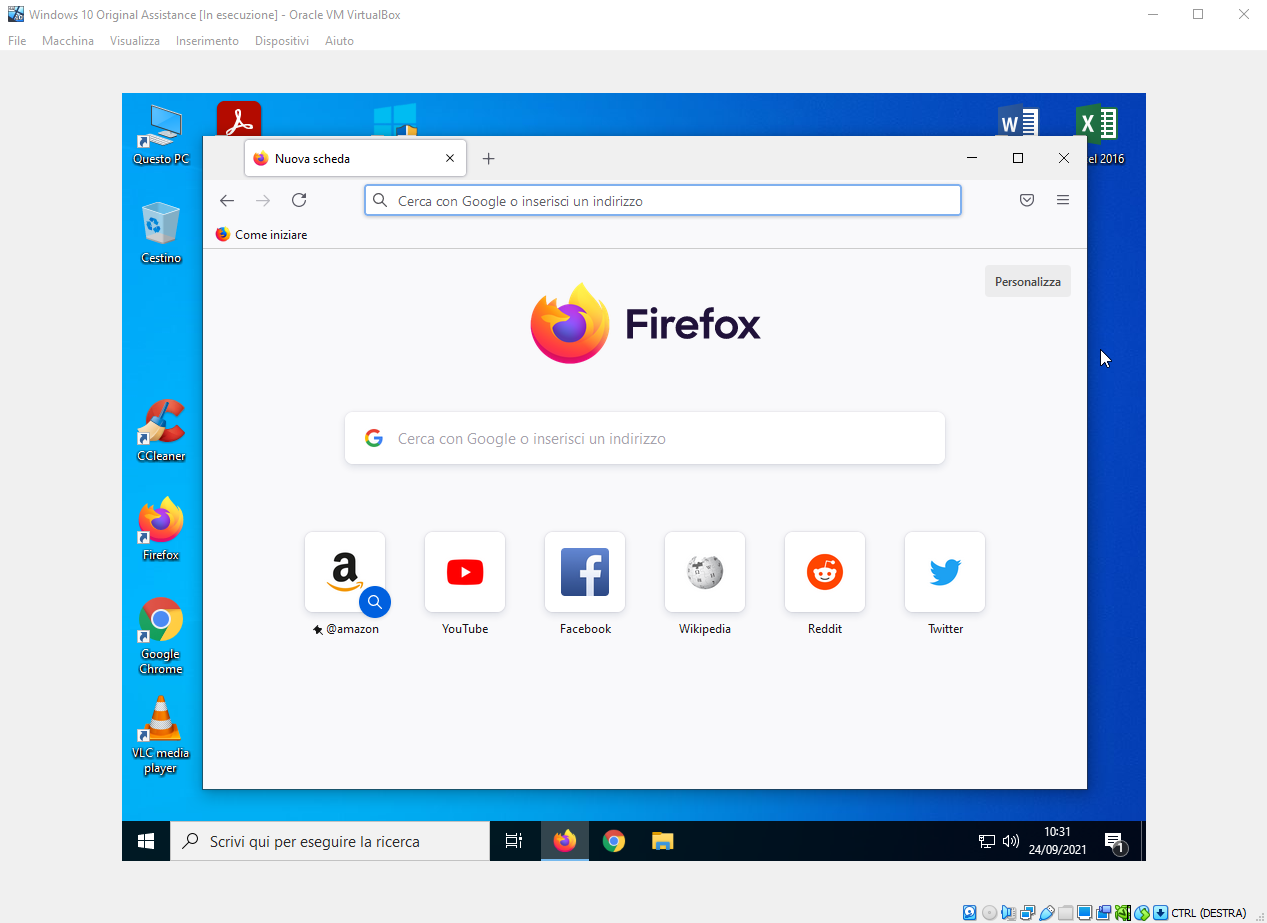
\includegraphics[width=0.6\columnwidth]{immagini/screenshot/firefox_virtualbox} 
    \caption{Browser "Firefox" virtualizzato tramite software di virtualizzazione "VirtualBox"}
\end{figure} \\

\begin{figure}[!h]     
\centering 
    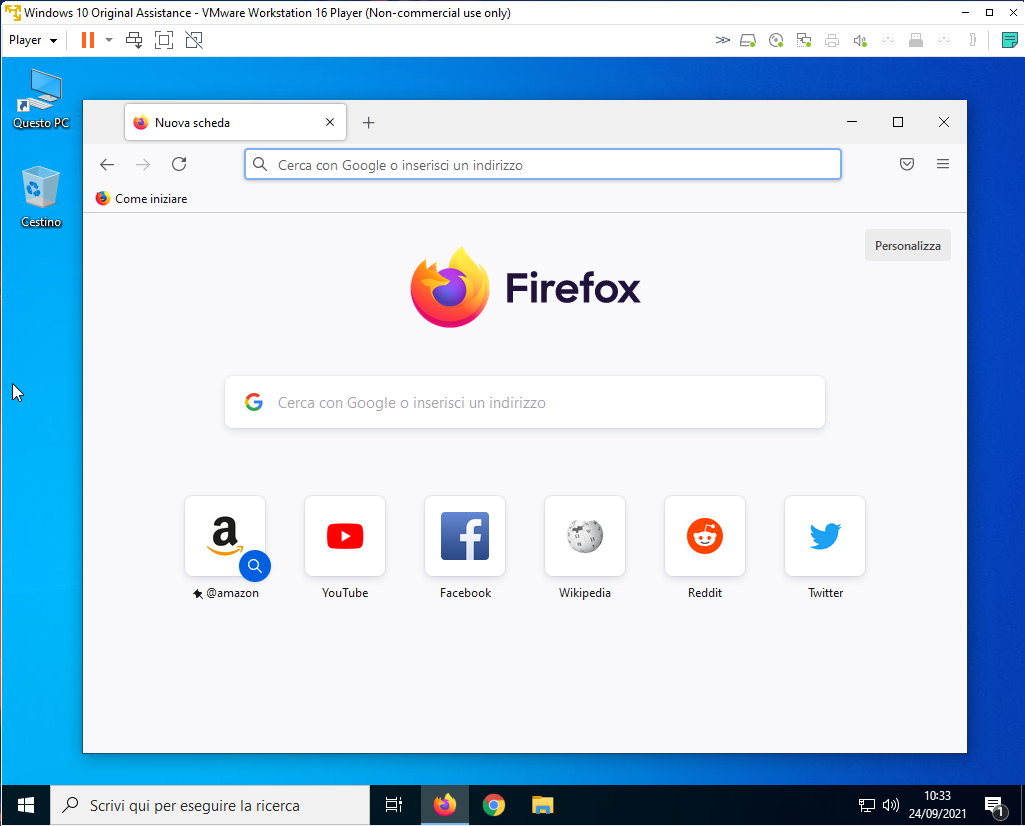
\includegraphics[width=0.6\columnwidth]{immagini/screenshot/firefox_vmware} 
    \caption{Browser "Firefox" virtualizzato tramite software di virtualizzazione "VMWare"}
\end{figure}

\newpage
Al fine di permettere al sistema operativo \textit{host} la virtualizzazione di uno o più sistemi operativi, è necessario installare un \textit{\gls{hypervisor}}\footcite{installabile solamente se il processore supporta la virtualizzazione e se quest'ultima e' abilitata da BIOS}, \textit{native} o \textit{hosted}, ovvero uno strato software che si interfacci e gestisca tutte le \textbf{istanze} di macchine virtuali in esecuzione sulla macchina locale. \\
La virtualizzazione non è priva di svantaggi. Il primo tra tutti, è appunto la necessità di dover \textit{virtualizzare} un intero sistema operativo al fine di eseguire l'applicativo virtuale desiderato.
Questo vincolo obbligatorio implica un consumo di memoria \gls{RAM} e di \gls{storage} non indifferente anche solo per eseguire il singolo sistema operativo virtualizzato \textbf{senza alcuna} applicazione virtuale in esecuzione.
Ne consegue quindi, che un'architettura a macchine virtuali avrà bisogno di uno spazio di \textit{storage} e di un quantitativo di memoria \textit{RAM}\footcite{il tipo di RAM "ECC" risulta preferibile ma non obbligatorio} installata sul server non indifferente. Anche in termini di consumo \textit{\gls{CPU}}, la virtualizzazione di molteplici sistemi operativi con le relative applicazioni virtualizzate in esecuzione può comportare \textbf{grossi carichi prestazionali} al server fisico, in quanto la CPU dell'host dovrà servire ed eseguire ogni sistema operativo di \textbf{ogni istanza} di virtualizzazione.\\
Dal punto di vista della sicurezza, quando si virtualizza un sistema operativo, sia nella virtualizzazione \textit{native} che \textit{hosted}, alcuni registri CPU sono direttamente esposti alla macchina virtuale come, ad esempio, i registri \textbf{VT-x} e \textbf{VT-d} del processore\footcite{e' necessario abilitare le estensioni di virtualizzazione da BIOS della scheda madre.} \footcite{nel caso di architettura avente processori Intel, IOMMU per architetture basate su processori AMD.}. Questi registri permettono al processore di non rendere accessibile la totalità dei suoi registri all'\textbf{hypervisor} e di controllare le chiamate dirette al \textit{\gls{DMA}} da parte delle soluzioni software virtualizzate.\\
Relativamente alla condivisione della rete tra macchine virtuali e host fisico, nel caso in cui si fosse installato un commutatore di rete virtuale di tipo \textbf{\gls{NAT}}, la scheda di rete dell'host e il relativo traffico sarebbe \textbf{esposta} a tutto il set applicativo virtualizzato e viceversa, con conseguente mancanza di isolamento tra macchine virtuali stesse ed \textit{host} fisico. Ne conseguirebbe quindi, che eventuali condivisioni di rete, o connessioni applicative, sarebbero disponibili a \textbf{tutto il set} di macchine virtuali. \\
Una possibile soluzione a questo problema potrebbe essere il passaggio da commutatore virtuale di tipo \textit{NAT} ad un commutatore virtuale che riesca ad isolare le singole macchine virtuali tra di esse e l'\textit{host} fisico, anche, nel caso più estremo, assegnando ad ogni macchina virtuale una \textbf{propria scheda di rete} ed una \textbf{propria} \textit{\gls{VLAN}} di rete dedicata\footcite{per creare o impostare una VLAN, fare riferimento al router/firewall o allo switch di rete}.\\
Virtualizzare un intero sistema operativo implica, come abbiamo appena analizzato, un \textbf{elevato consumo di risorse fisiche}, specialmente nel caso in cui, per esigenze lavorative, si debba ricorrere ad una multipla virtualizzazione di sistemi operativi dove, in ognuno di essi, viene eseguita una specifica applicazione che deve essere accessibile ad altri \textit{client}.\\
Uno dei principali aspetti positivi di un'architettura a container sta proprio nel poter virtualizzare (o \textit{containerizzare} nel caso appunto di container) una singola e specifica applicazione \textbf{senza la necessità di inglobare un intero sistema operativo} nell'immagine virtuale. L'esecuzione dell'applicativo, nonostante appunto la mancanza di un sistema operativo, sarà comunque possibile grazie a chiamate di sistema al kernel del sistema operativo \textit{host}. Ne consegue quindi, che il container applicativo risultante di un'applicazione \textit{containerizzata} è di gran lunga di \textbf{dimensione inferiore} rispetto all' immagine\footcite{inteso come dimensione in Gb del virtual disk image (*.vdi) dell'immagine virtualizzata} della stessa applicazione \textit{virtualizzata}, causa appunto, in primis, mancanza di sistema operativo.\\
Un container è quindi una \textbf{singola unità atomica} contenente l'applicativo (il programma \textit{containerizzato}) con i relativi file atti alla sua corretta esecuzione senza l'immagine di un sistema operativo completo.
Al momento dell'esecuzione del container, l'applicazione \textit{containerizzata} verrà eseguita immediatamente sopra lo stato del sistema operativo \textit{host}, attraverso l'aiuto del \textbf{\gls{Docker Engine}}, senza alcun \textit{\gls{hypervisor}} come, ad esempio, nel caso dell'architettura a macchine virtuali. \\
Una rappresentazione grafica del concetto appena descritto è data dalla seguente immagine:
\begin{figure}[!h]     
\centering 
    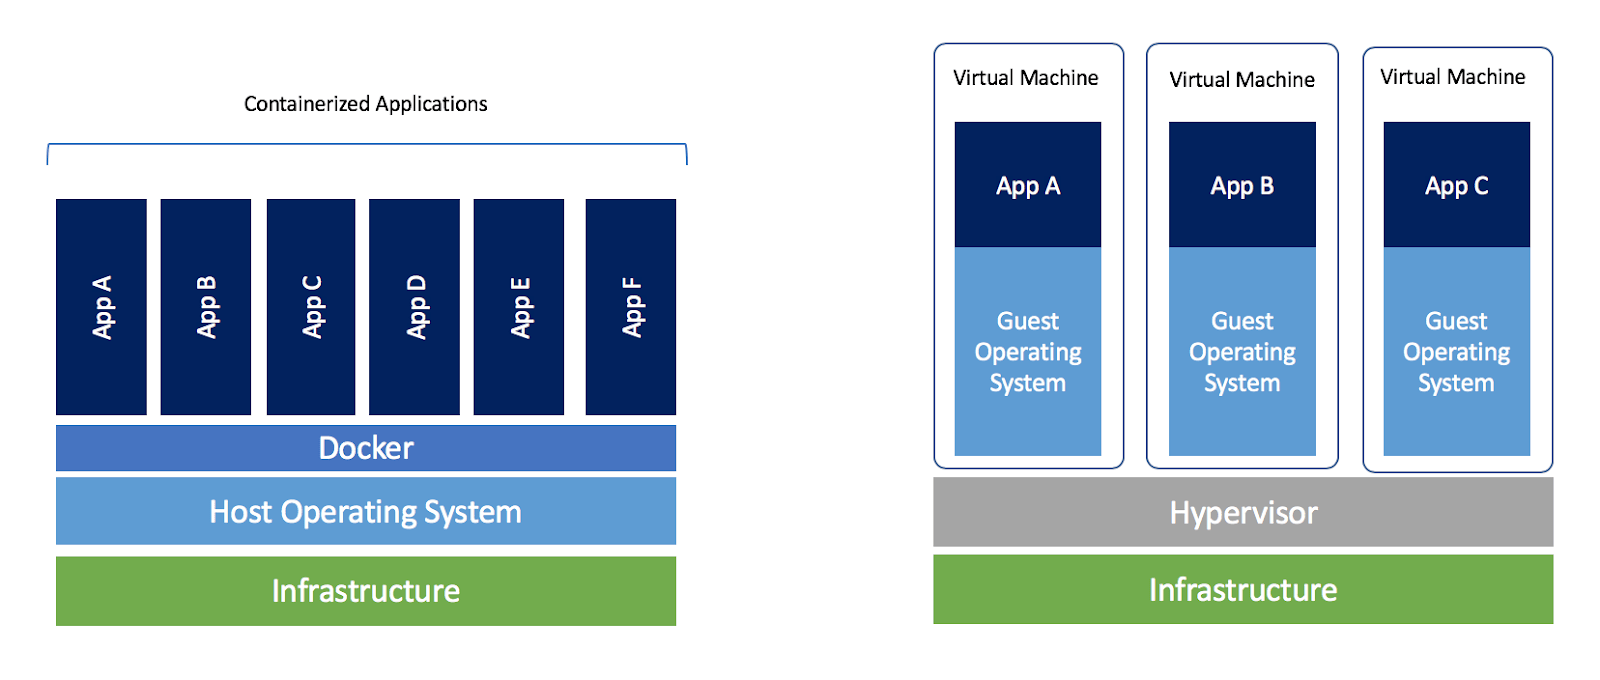
\includegraphics[width=0.6\columnwidth]{immagini/img/container_vs_vm} 
    \caption{Rappresentazione grafica dell'architettura a container ed a macchine virtuali}
\end{figure} \\
%TODO: immagine a layer raffgurante container vs virtual machine.
\\Un'architettura a \textbf{container} infatti, a differenza dell'architettura a macchine virtuali, garantisce un'esecuzione \textbf{separata} e \textbf{protetta} di \textbf{ogni singolo applicativo} compatibile con il sistema operativo host, indipendentemente dal numero di container presenti nel sistema o dal tipo di interfaccia di rete. \\
E' possibile, inoltre, far coesistere multipli container di uno stesso applicativo in esecuzione nello stesso momento (anche sfruttando il \textit{\gls{load-balancing}}, come si accennerà nel corso di questa tesi) assegnandoci, esattamente come con le macchine virtuali, eventuali \textbf{indirizzi IP} statici, \textbf{CPU limit} e \textbf{disk quota}.\\
Essendo un container una \textbf{\gls{sandbox}} applicativa indipendente dal sistema operativo, i dati generati dalla sua esecuzione sono destinati a scomparire nell'eventualità in cui il container venisse distrutto. Per ovviare a questo problema, si può ricorrere ad una tecnica di \textbf{volume-mapping}, ovvero una tecnica che permette di esporre il \textbf{\gls{filesystem}} interno al container permettendone quindi la \textbf{lettura e scrittura} direttamente da parte dell'\textit{host}. La tecnica appena accennata sarà trattata in maniera più approfondita nel corso della lettura di questa tesi.\\
Godendo i container di un approccio standardizzato per la loro costruzione ed esecuzione, è quindi di facile intuizione la facilità di \textit{portabilità} di questi. Un container, infatti, può essere distribuito su una nuova piattaforma in maniera estremamente veloce e senza alcuna modifica allo stesso. Ne consegue, che un eventuale \textbf{rilascio e distribuzione} di un applicativo interno ad un container può essere molto velocizzato rispetto alla stessa operazione svolta invece su un'architettura a macchine virtuali. Relativamente sempre allo sviluppo e distribuzione di un applicativo, tramite container è possibile un controllo di versione dell'applicativo stesso più flessibile: è possibile infatti gestire le versioni del codice con le relative dipendenze inglobando il tutto in un unico container, formando quindi un' unità atomica di più facile manutenzione e distribuzione. Un eventuale ripristino o \textbf{\gls{rollback}} delle modifiche potrà essere facilmente eseguito tramite \textbf{ripristino in esecuzione} del container contenente le modifiche precedentemente effettuate dal team.\\
Un altro dei vantaggi decisivi di un'architettura a container è la sua facilità di gestione. L'avvio, rimozione o la duplica dei container è un'operazione decisamente \textbf{meno onerosa} rispetto alla controparte nelle macchine virtuali (basti solo pensare al tempo di \textit{\gls{boot}} del sistema operativo), e può essere \textbf{facilmente automatizzata e gestita} dal Docker Engine. Ne consegue quindi, che la \textbf{scalabilità}, ovvero la facilità di modifica dell'infrastruttura per far fronte alle variazioni di mole di informazioni trattate o carichi di lavoro, risulta di \textbf{gestione più semplice} anche per la figura sistemistica interna all'azienda.
\\
La presente immagine ritrae il browser web "Mozilla Firefox" in esecuzione all'interno di un container esposto all'\textit{host} nella porta 5800:
\begin{figure}[!h]     
\centering 
    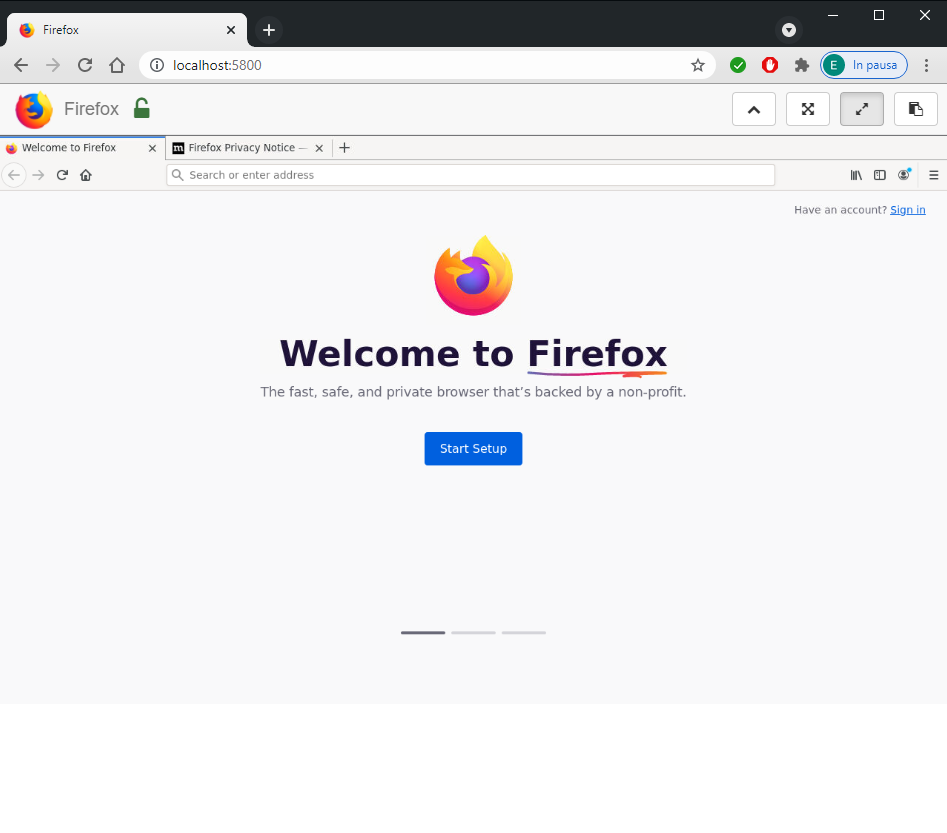
\includegraphics[width=0.6\columnwidth]{immagini/screenshot/firefox_container} 
    \caption{Browser web "Firefox" in esecuzione su un container con porta 5800 esposta all'host}
\end{figure} \\
%\begin{figure}[h!]
%    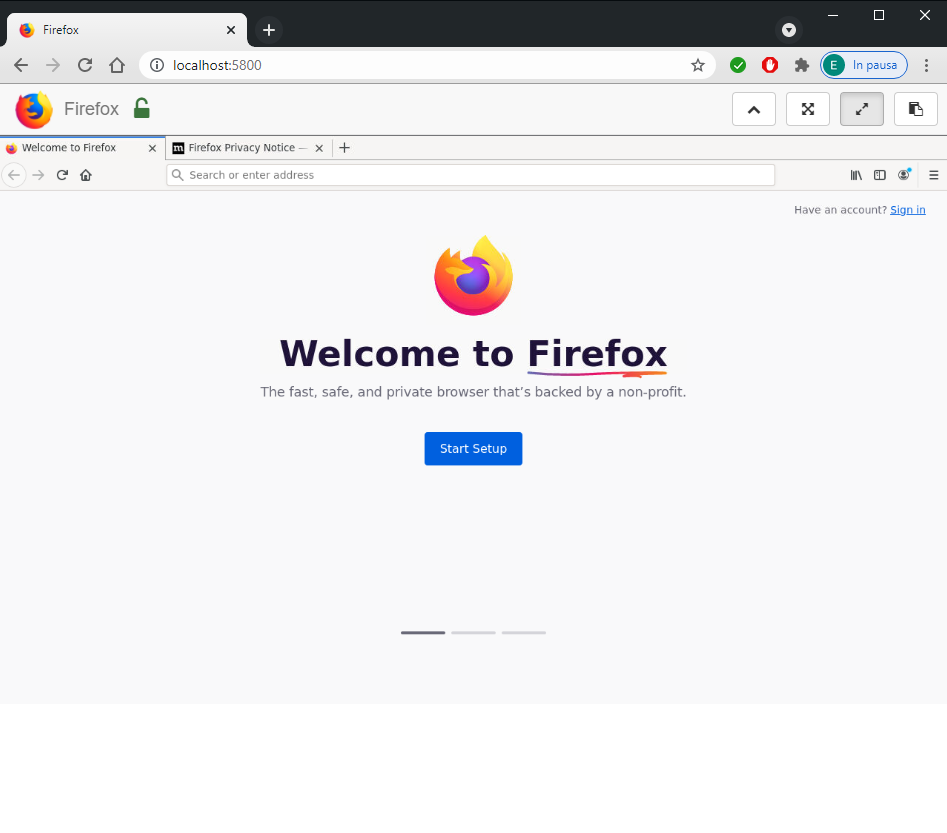
\includegraphics[width=1\textwidth]{./immagini/screenshot/firefox_container.png}
%    \caption{Applicativo "Firefox" in esecuzione su un container all'interno del browser web "Chrome"}
%\end{figure}
%TODO: come si ottiene un container (immagine s.o. + applicazione) vs come si ottiene lo stesso con una macchina virtuale.
\newpage
\section{Analisi di Docker: architettura e funzionalità}

Una delle piattaforme di riferimento più utilizzate e supportate in ambito container è appunto \textbf{Docker}. Nato dall'azienda dotCloud nel 2003 e pubblicato successivamente come progetto \textbf{\gls{open-source}}, è una piattaforma atta alla gestione dei container. Tramite \textbf{Docker Desktop}\footcite{presente solamente per le versioni Windows}, è possibile monitorare, avviare, arrestare e gestire eventuali container creati. \\
Come già anticipato nel corso di questa tesi, Docker lavora a stretto contatto con il suo motore, ovvero \gls{Docker Engine}, che si occupa appunto della \textbf{creazione} e \textbf{manutenzione} dei container nel sistema.
Il \textit{Docker Daemon} è il processo principale di Docker, cui compito è appunto la gestione e l'orchestrazione dei container nel sistema operativo dove è installato. \\
Al momento della creazione di un nuovo container, questo processo interroga i \textit{Docker Registries} per verificare la presenza di una immagine già pronta all'uso del programma che si vuole \textit{containerizzare}. I Docker Registries sono un insieme di immagini di container \textbf{pronte all'uso} e \textbf{scaricabili gratuitamente} da qualunque client Docker. Queste immagini sono create e manutenzionate dalla \textbf{Docker Community}, e permettono allo sviluppatore di avere delle immagini (o \textit{layer}) già pronti, testati e funzionanti al fine di costruire con successo la propria immagine di applicativo virtuale. Il Docker Registries più comune ed utilizzato è "\textbf{DockerHub}".\\
Come già menzionato nel corso di questo documento, tramite Docker è possibile costruire delle immagini di un applicativo virtuale. Un' immagine è un \textbf{set di comandi} cui scopo è quello di creare, una volta eseguito, un container. Un' immagine può basarsi, a sua volta, su altre immagini, ed il set di comandi che espandono l'immagine sorgente compongono, a loro volta, la nuova immagine applicativa. I comandi atti alla corretta costruzione della stessa vengono scritti su un apposito file, chiamato appunto "\textbf{dockerfile}", ed ogni comando (riga del file) si traduce in un nuovo \textit{layer} della nuova immagine. Un \textbf{dockerfile} è un documento di testo, senza alcuna estensione, contenente una serie di passi ed istruzioni atti alla \textbf{corretta creazione} di un' immagine di un applicativo. Il Docker Daemon, per costruire correttamente un' immagine, leggerà ed eseguirà in maniera \textbf{sequenziale} ogni comando trascritto all'interno del \textit{dockerfile}, ed al termine della lettura dello stesso, si avrà un'immagine eseguibile di un applicativo. \\
Un \textbf{container} è un'\textbf{istanza di esecuzione} di un'immagine a cui è attribuito un nome, arbitrario o definito dal programmatore, attraverso il Docker Daemon. 

%Tramite Docker è quindi possibile l'organizzazione e orchestrazione di tutti i container applicativi installati sul client.


\section{Creazione di container vs creazione di VM}

La creazione di una VM è possibile tramite apposito \textit{hypervisor}. Tuttavia, al momento della creazione, l'utente deve essere a conoscenza della quantità massima di risorse \textit{hardware} da destinare alla stessa. Questa stima, oltre ad includere il costo\footcite{inteso come quantitativo di risorse fisiche da allocare} richiesto dal programma da \textit{virtualizzare} che si andrà ad installare all'interno della VM, deve includere anche il costo, almeno soddisfacente i requisiti minimi, relativo al sistema operativo. 
%La seguente schermata rappresenta la creazione della macchina virtuale con 8Gb di RAM e 80Gb di disco rigido dedicati:\\
%TODO: immagine di avvio dell'installazione di Windows 10 Pro da VMWARE
Terminata la fase di \textbf{analisi dei costi}, sarà necessario installare \textbf{manualmente} il sistema operativo all'interno della macchina virtuale appena creata. Per fare ciò, bisognerà avviare la macchina virtuale da un supporto di \textbf{boot}, come ad esempio una immagine \gls{ISO} avviabile di un sistema operativo.
Successivamente alla fase di avvio di installazione della VM, si passerà alla fase vera e propria di installazione del sistema operativo.%, riassunta nelle seguenti immagini:
%TODO: immagini dell'installazione del sistema operativo nella VM con VMWARE.
Una volta ottenuta un'installazione funzionante ed avviabile, per ottimizzarne al meglio le prestazioni, tramite ad esempio installazione dei relativi \gls{driver} video virtuali, ed espanderne le funzionalità, come la possibilità di accedere a \textit{volume-mapping} condivisi con il sistema operativo \textit{host}, è necessario installare le relative \textbf{\gls{guest additions}}, proprie di ciascun programma di virtualizzazione.
%TODO: immagine raffigurante l'installazione delle Guest Additions su VMWARE.
Una volta fatti i passi sopra-descritti, si avrà un sistema operativo virtualizzato completamente funzionante, pronto per l'installazione di tutto il software applicativo desiderato.
%TODO: immagine raffigurante W10 Pro avviato e funzionante con Firefox in esecuzione.
\\
Come precedentemente affermato, un container è un'unità atomica costituita principalmente da una o più applicazioni e dalle librerie di sistema operativo atte al loro corretto funzionamento.
Al fine di poter generare ed utilizzare prima un'immagine applicativa e successivamente un container, è necessario prima costruirne il relativo \textbf{\gls{dockerfile}}.
Ogni \textit{dockerfile} di ogni immagine applicativa contiene un set di istruzioni e comandi atti alla corretta installazione e configurazione dell'applicativo virtuale. Ogni comando scritto nel \textit{dockerfile} comporrà un nuovo \textit{layer} del container.
%Le seguenti immagini mostrano i corretti passi per la costruzione di un container con, all'interno, l'applicativo "Firefox":
%TODO: immagini raffiguranti i passi e comandi atti alla creazione di un container
La creazione di multipli container cloni, ovvero container generati da una singola immagine, è un'operazione di semplice e veloce esecuzione, in quanto il Docker Engine, durante la costruzione di ogni container, adotta un meccanismo di \textit{\gls{caching}} dei vari \textit{\gls{layer}} di cui un container è composto. Questo meccanismo permette quindi una costruzione, o aggiornamento, di un container \textbf{molto più veloce} rispetto ad una sua completa ri-creazione, in quanto si useranno, se compatibili, i layer in cache già \textbf{precedentemente costruiti} al fine di costruire il nuovo container contenente l'applicativo, nuovo o aggiornato, desiderato.\\
Durante tutta la durata dello stage si è utilizzata la piattaforma "Docker" per la creazione delle varie immagini e container per gli applicativi specificati nel sommario e nell'introduzione.

\section{Installazione di Docker in ambiente Windows}
Al fine di poter creare ed orchestrare dei container, è necessaria l'installazione del software "\textbf{Docker Desktop}" nel proprio computer. Docker Desktop è compatibile con tutte le versioni di Windows a partire da Windows 10 Home (build 19041), ed i requisiti minimi sono i seguenti:
\begin{itemize}
	\item Processore a \textbf{64 bit};
	\item 4Gb di memoria \textbf{RAM};
	\item Virtualizzazione hardware abilitata da \textbf{\gls{BIOS}};
	\item Funzionalità \textbf{Hyper-V} abilitata da Windows \footcite{Per abilitare il supporto di virtualizzazione Hyper-V su Windows bastera' entrare nell'apposito menu "Abilita o disabilita funzionalità di Windows" e selezionare la voce "Hyper-V"}.
\end{itemize}

%TODO: immagine mostrante l'abilitazione della funzionalità Hyper-V su Windows.
Una volta scaricato l'\gls{installer} di Docker Desktop, l'installazione è una procedura relativamente semplice, in quanto è del tipo "\textbf{one click-install}".\\
Durante tutta l'installazione è necessaria una connessione ad internet attiva.\\
Terminata l'installazione, per avviare Docker Desktop basterà aprire il menu \textbf{Start} di Windows e cliccare sulla relativa icona di Docker Desktop come nell'immagine:\\
\begin{figure}[!h]     
\centering 
    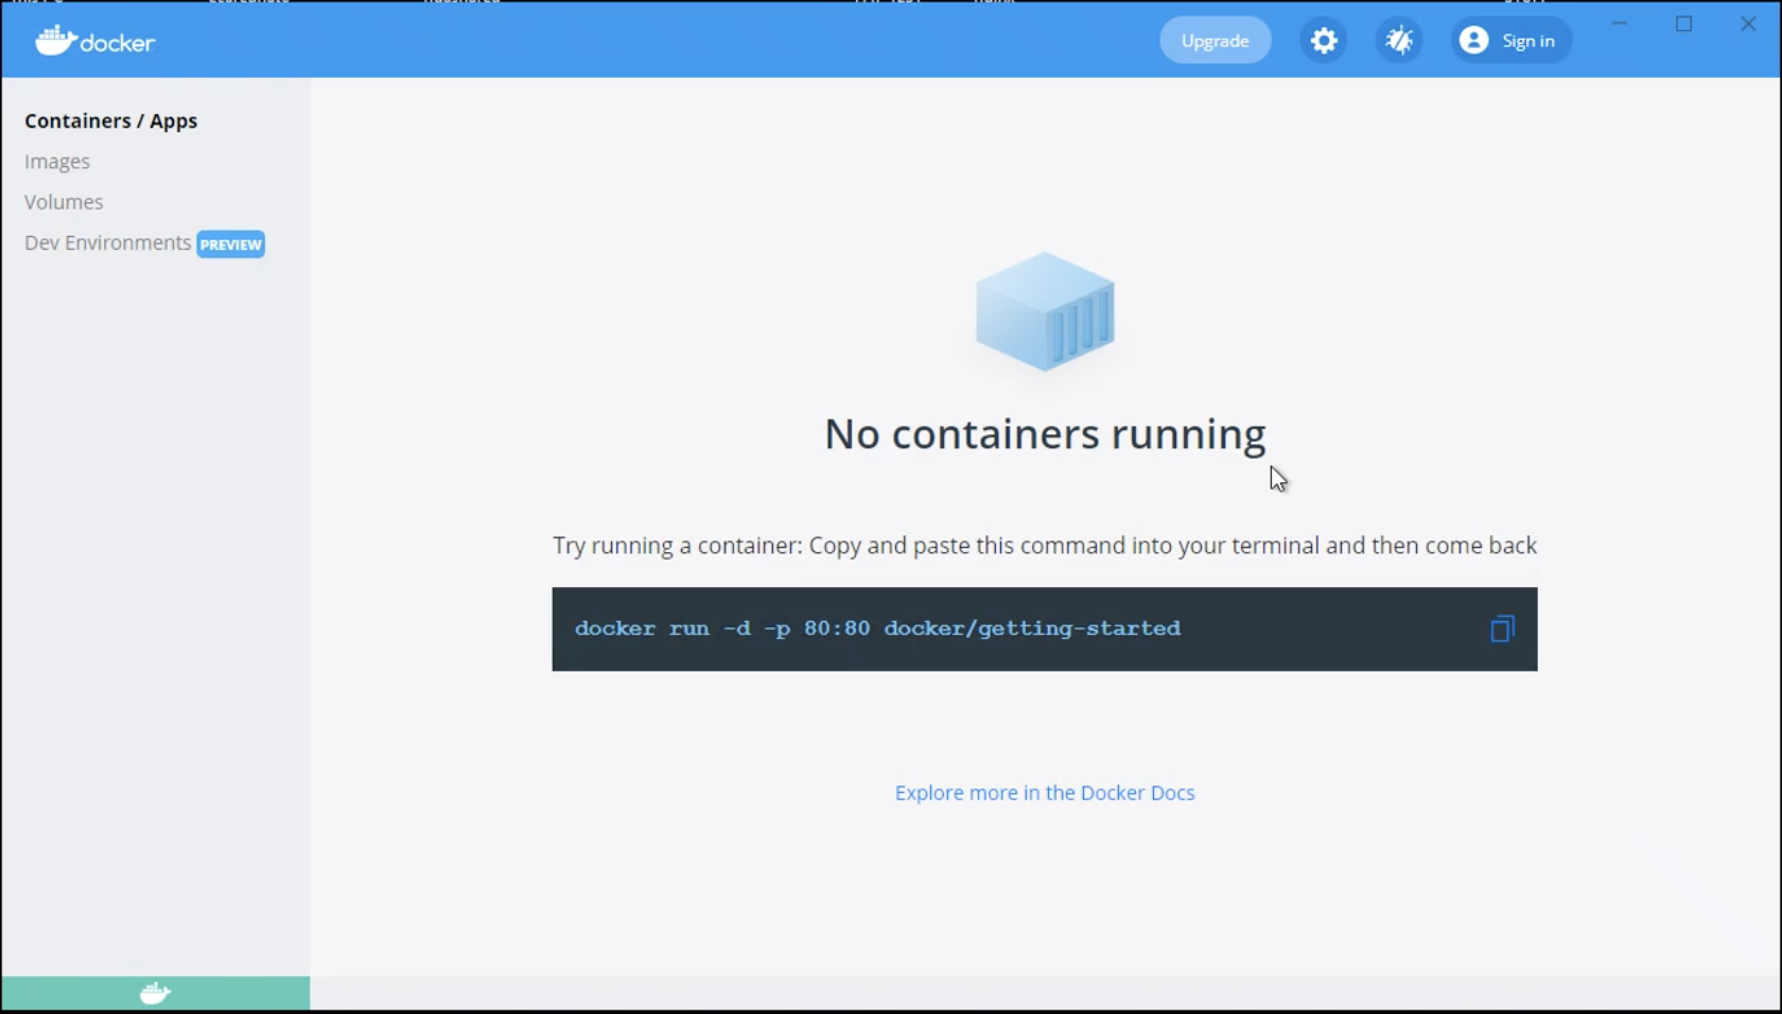
\includegraphics[width=1.0\columnwidth]{immagini/screenshot/docker_desktop_initialscreen} 
    \caption{Schermata principale di "Docker Desktop" con nessun container in esecuzione}
\end{figure} \\

%TODO: immagine mostrante l'icona di Docker Desktop presente nel menu Start di Windows terminata l'installazione.

             % Kick-Off
% !TEX encoding = UTF-8
% !TEX TS-program = pdflatex
% !TEX root = ../tesi.tex

%**************************************************************
\chapter{Analisi composizione e costruzione container}
\label{cap:analisi-container}
%**************************************************************

\intro{Breve introduzione al capitolo}\\

\section{Composizione container}



\section{Dockerfile container: analisi struttura e spiegazione}

%\begin{figure}[!h] 
%    \centering 
%    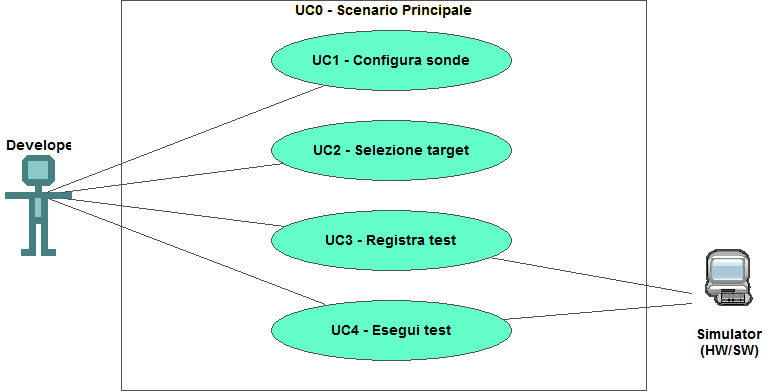
\includegraphics[width=0.9\columnwidth]{usecase/scenario-principale} 
%    \caption{Use Case - UC0: Scenario principale}
%\end{figure}

\section{Costruzione container tramite automazione: HDA Sandbox Builder}
             % Concept Preview
% !TEX encoding = UTF-8
% !TEX TS-program = pdflatex
% !TEX root = ../tesi.tex

%**************************************************************
\chapter{Orchestrazione container}
\label{cap:orchestrazione-container}
%**************************************************************

\intro{Breve introduzione al capitolo}\\
In questo capitolo verrà esplicata la metodologia di orchestrazione tra container adottata in Azienda, fornendo al lettore, in primis, una panoramica su Docker Compose e, successivamente, l'integrazione dello stesso per la corretta costruzione di una \textit{sandbox} applicativa di HDA.
%**************************************************************
\section{Breve panoramica su Docker Compose}
\textbf{Docker Compose} è uno strumento per la gestione ed orchestrazione di applicazioni Docker \textbf{multi-container}. In un ambiente costituito da multipli container in esecuzione, può essere relativamente \textbf{difficile} e \textbf{gravoso} per l'utente manutenzionare, avviare o fermare multipli container. Per aiutare appunto nell'orchestrazione, intesa come \textbf{monitoraggio}, \textbf{avvio}, \textbf{ri-avvio} in caso di \textit{failure} ed \textbf{arresto} di multipli container, l'utente può installare Docker Compose sulla propria workstation, per centralizzare così la gestione di tutti i container da un'unica interfaccia.\\
Tramite definizione di un file \textbf{YAML} (ex: \textit{docker-compose.yml}), si può istruire Docker Compose relativamente a quali container dovrà avviare specificando, inoltre, eventuali parametri aggiuntivi, quali \textit{volume-mapping} o interfacce di rete aggiuntive.\\
I passi che Docker Compose esegue per creare quindi la \textit{sandbox} applicativa di HDA sono i seguenti:
\begin{itemize}
	\item \textbf{lettura} del file docker-compose.yml;
	\item \textbf{lettura}, ricorsiva, dei \textbf{dockerfile} relativi ai \textbf{container} definiti nel docker-compose.yml;
	\item \textbf{costruzione}, secondo l'ordine ed eventuali parametri definiti nel docker-compose.yml, delle \textbf{immagini} dei container dichiarati nel Compose-file (docker-compose.yml).
\end{itemize}
Una volta costruite tutte le immagini dei container propri della \textit{sandbox} applicativa di HDA, è possibile lanciare la \textit{sandbox} applicativa tramite il semplice comando: \centerline{\textbf{[docker-compose
-f docker-compose.yml -p nomecliente up]}} sostituendo "nomecliente" con il nome effettivo del cliente \textbf{proprietario} della \textit{sandbox} di HDA. I parametri \textbf{-f} e \textbf{-p} definiscono, rispettivamente, la possibilità di dichiarare un Compose-file alternativo e la possibilità di assegnare un nome alternativo all'istanza, la quale, di \textit{default}, acquisirebbe il nome della directory contenente il Compose-file.

%\label{sec:tecnologie-strumenti}

%\subsection*{Tecnologia 1}
%Descrizione Tecnologia 1.

%**************************************************************
\section{Docker compose per la costruzione di una sandbox applicativa}
Come visto nel paragrafo precedente, tramite Docker Compose è possibile orchestrare l'avvio e l'arresto di una intera \textit{sandbox} applicativa di HDA tramite un \textbf{singolo comando}. Tramite l'uso di Docker Compose, l'esecuzione \textbf{simultanea} di più \textit{sandbox} applicative di HDA risulta di semplice esecuzione, in quanto basterà lanciare nuovamente il comando descritto nel paragrafo precedente per creare una nuova \textit{sandbox} applicativa destinata ad un altro cliente. \\
Ogni \textit{sanbdbox} ha un nome, il quale deve necessariamente essere \textbf{univoco}.
La seguente immagine mostra una panoramica, fornita da Docker Compose, di due \textit{sandbox} applicative, con i relativi container di cui composte, in esecuzione \textbf{simultanea} sullo stesso \textit{host}, chiamate rispettivamente \textit{nomecliente} e \textit{cliente2}:
\begin{figure}[!h]     
\centering 
    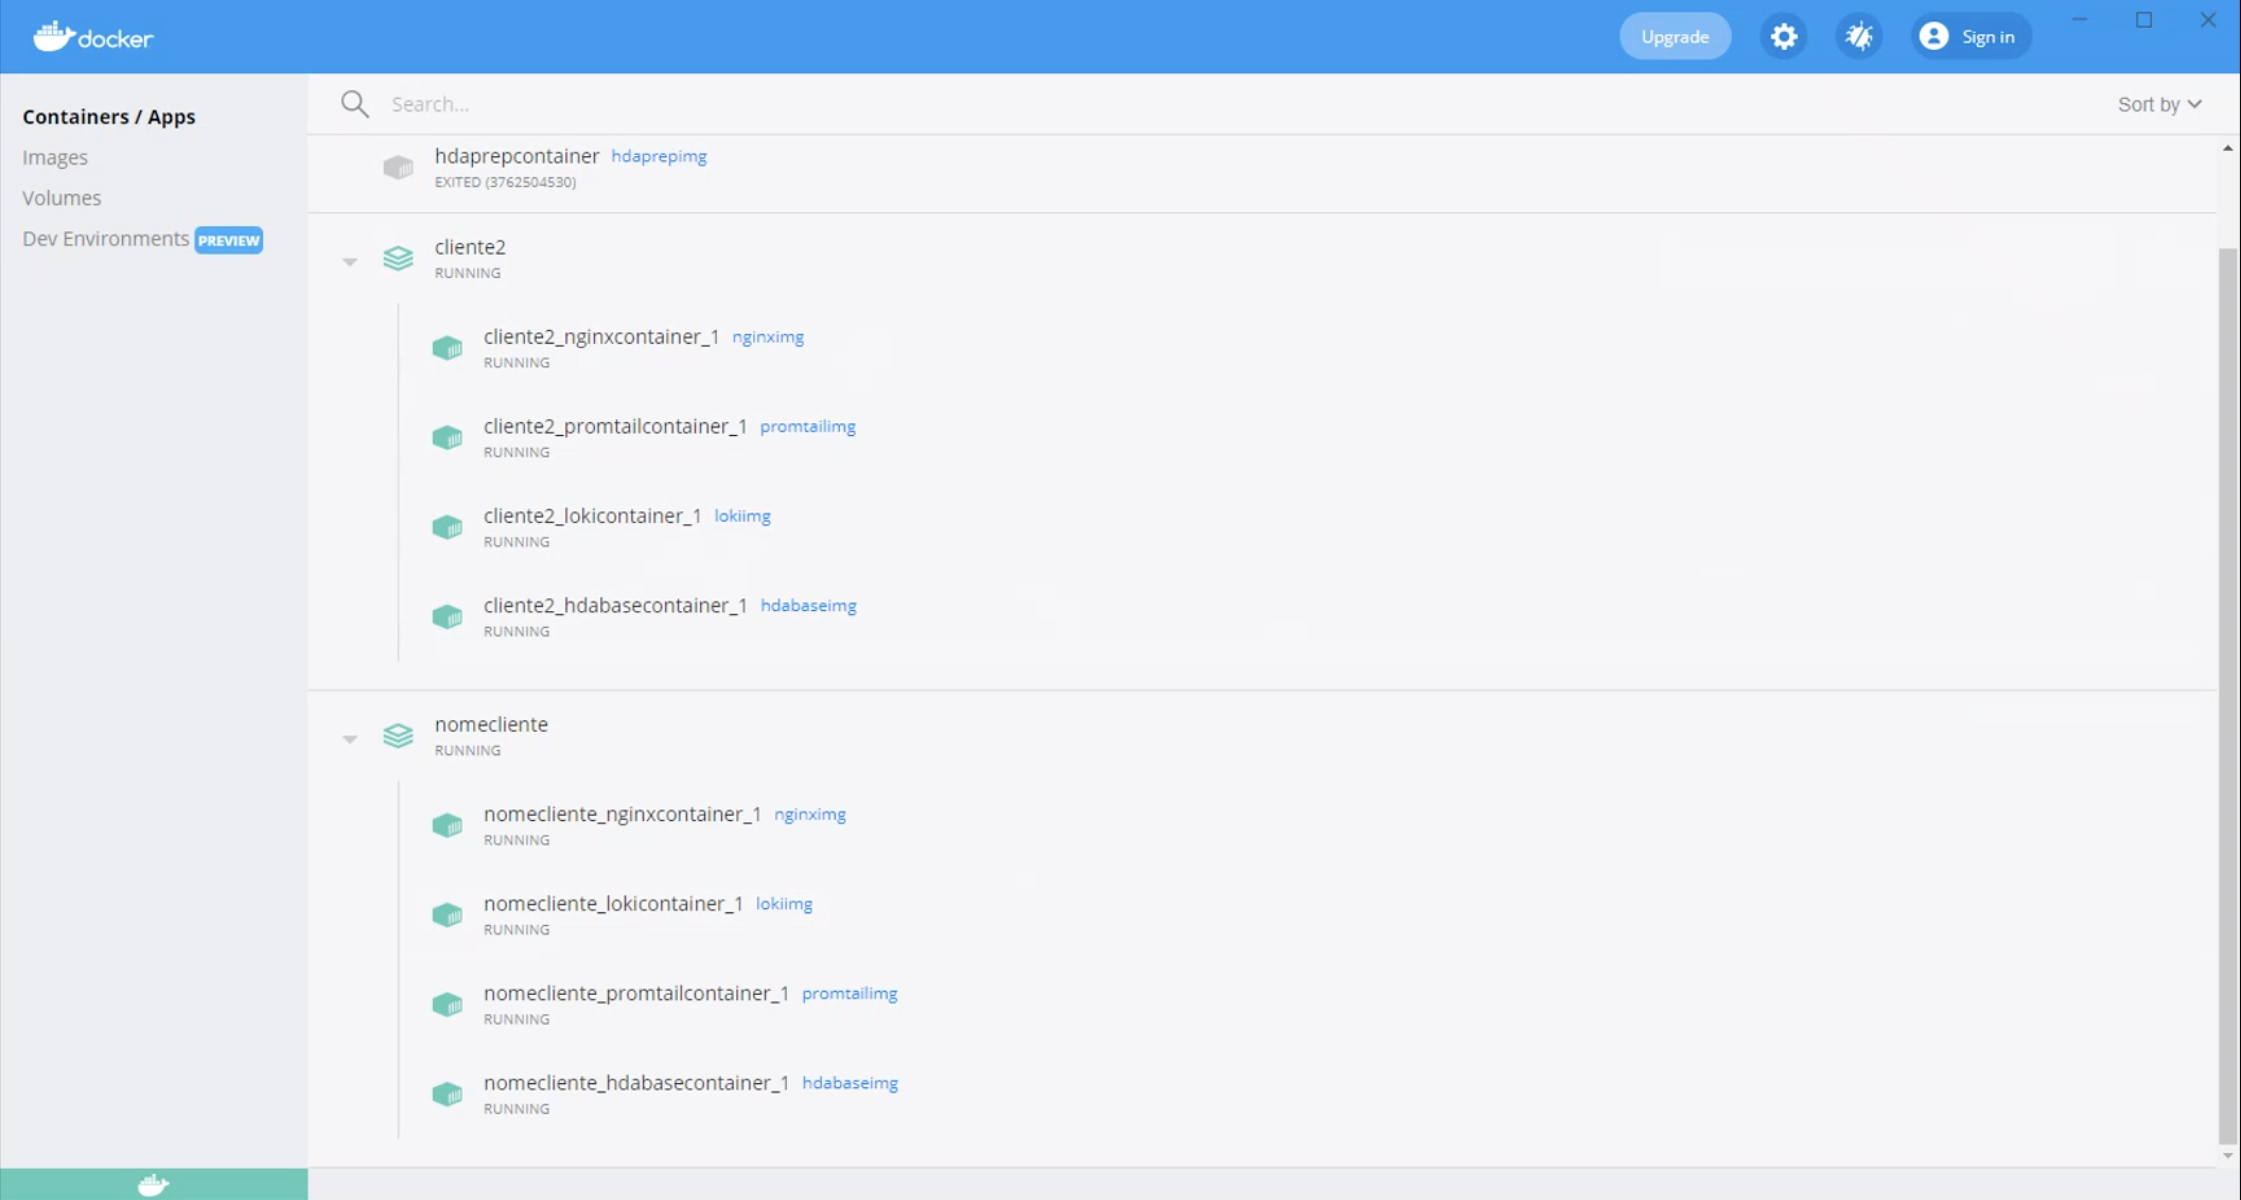
\includegraphics[width=1.0\columnwidth]{immagini/screenshot/docker_compose_sandbox} 
    \caption{Interfaccia di Docker Compose con in esecuzione due \textit{sandbox} applicative}
\end{figure} \\
%\subsubsection{Namespace 1} %**************************
%Descrizione namespace 1.


%**************************************************************
\section{Integrazione di HDA Sandbox Builder con Docker Compose}
Come visto all'interno di questo capitolo, tramite Docker Compose è possibile la costruzione delle immagini relative ai container che comporranno, successivamente, una volta lanciati in esecuzione, la \textit{sandbox} applicativa di HDA. Per arrivare ad una corretta esecuzione di una \textit{sandbox} applicativa però, la costruzione tramite Docker Compose dei container stessi che la compongono \textbf{non è sufficiente}. E' il caso, ad esempio, del container atto alla preparazione del filesystem di HDA ("hdaprepcontainer"), senza il quale l'istanza di HDA \textbf{non riuscirà ad avviarsi} a causa di un \textit{settaggio} errato dei permessi nella cartella \textbf{/App\_Data} dello stesso. Questo container non è inserito all'interno all'interno del Compose-file, in quanto deve essere \textbf{manualmente lanciato e supervisionato} dall'utente installatore, e l'esecuzione del container dovrà terminare \textbf{prima} di poter lanciare una qualsiasi \textit{sandbox} applicativa di HDA. Anche il container "hdadbupdatercontainer" è escluso dal Compose-file, in quanto, anch'esso, dovrà essere \textbf{eseguito manualmente} dall'utente installatore e continuamente supervisionato durante la sua completa esecuzione.\\
E' quindi facilmente intuibile, che l'esecuzione di Docker Compose dovrà essere necessariamente \textbf{subordinata} all'esecuzione del \textit{batch-file} \textbf{HDA\_sandbox\_builder.bat}.\\
Riassumendo, i passi atti ad una corretta esecuzione di una \textit{sandbox} applicativa di HDA sono i seguenti:
\begin{itemize}
	\item \textbf{Passo 1:} lancio del \textit{batch-file} \textbf{HDA\_sandbox\_builder.bat}, con costruzione ed esecuzione \textbf{obbligatoria} del container "hdaprepcontainer";
	\item \textbf{Passo 2:} creazione di una directory avente nome del cliente stesso che conterrà il \textit{filesystem} della nuova \textit{sandbox} applicativa di HDA generato dal passo precedente;
	\item \textbf{Passo 3:} da prompt dei comandi con privilegi di amministratore, lanciare il comando "\textbf{xcopy}" relativamente ai file situati nella cartella App\_Data del container "hdaprepcontainer", situato all'interno della directory creata al punto precedente;
	\item \textbf{Passo 4:} esecuzione del comando di Docker Compose "\textbf{docker-compose-f docker-compose.yml -p nomecliente up}" sostituendo al posto della stringa "nomecliente" il \textbf{nome del cliente scelto} nel passo 2.
\end{itemize}
L'obbligatorietà dell'esecuzione manuale di questi quattro distinti passi è stata \textbf{strettamente voluta dall'Azienda}, in quanto ha preferito non automatizzare l'intera procedura di creazione di una \textit{sandbox} applicativa per avere un maggior controllo in ogni "passo" della sua creazione.\\
Il corretto instradamento degli accessi da parte degli utenti alle istanze di HDA contenuta nel relativo container ("hdabasecontainer") all'interno delle \textit{sandbox} applicative sarà trattato nel prossimo capitolo.







%**************************************************************             % Product Prototype
% !TEX encoding = UTF-8
% !TEX TS-program = pdflatex
% !TEX root = ../tesi.tex

%**************************************************************
\chapter{Reverse Proxy tramite NGINX sulle sandbox di HDA}
\label{cap:nginx-reverse-proxy}
\intro{Breve introduzione al capitolo}\\
In questo capitolo verrà esplicata la metodologia di \textbf{reverse-proxy} tra \textit{sandbox} applicative di HDA per premettere a diverse utenze esterne un accesso privato ad una singola istanza di HDA in esecuzione su un determinato host.

\section{Introduzione ad NGINX}
NGINX è un applicativo web-server multipiattaforma ad alte prestazioni, comunemente usato come reverse-proxy o load-balancer. Nato nel 2004 e progettato per garantire un basso consumo di memoria, utilizza un approccio asincrono, basato su \textit{event}, dove le richieste vengono gestite su un singolo thread. Ogni \textit{thread} worker, ovvero un processo che esegue un'elaborazione effettiva, è gestito da un \textit{thread} master, il quale lo coordina e lo controlla.\\
All'interno di Docker-Hub è presente un repository ufficiale, gestito dalla Nginx Foundations, contenente un'immagine ufficiale di NGINX basata sul sistema operativo Alpine Linux, ovvero una distribuzione Linux che ha fatto della leggerezza un requisito fondamentale. Come precedentemente spiegato in questo documento, il container atto al reverse-proxy automatizzato contenente un'immagine di NGINX è chiamato "nginxcontainer", e fa parte anch'esso della \textit{sandbox} applicativa di HDA.

\section{Logica di reverse-proxy su sandbox di HDA}
Affinchè un utente, interno od esterno alla \textit{intranet} aziendale, possa accedere al relativo container contenente l'istanza, personalizzata o meno, di HDA, è necessario che conosca il relativo \textbf{FQDN} della \textit{sandbox} applicativa di HDA alla quale si vuole accedere.\\
Un FQDN, acronimo di \textit{Fully Qualified Domain Name}, è un nome di dominio che specifica la posizione assoluta di un nodo (in questo caso, la nostra \textit{sandbox} applicativa di HDA) all'interno della gerarchia DNS. Un FQDN si distingue da un generico nome di dominio per l'aggiunta del nome dell'host nel prefisso della stringa di dominio, in modo tale da renderla univoca. Un esempio di FQDN di un container è facilmente visibile nell'immagine esplicante l'architettura del progetto nel capitolo 4.1.
Nonostante l'utente \textbf{non acceda in maniera diretta} al container contenente l'istanza di HDA, l'attributo FQDN di ogni container nelle relative \textit{sandbox} è assegnato in maniera automatica da Docker Compose secondo la seguente logica decisa assieme all'Azienda:
\centerline{\textbf{nomecliente\_nomecontainer\_numeroistanza}}
dove:
\begin{itemize}
	\item \textbf{nomecliente} identifica il nome della \textit{sandbox} applicativa a cui il container appartiene. Generalmente, il nome della \textit{sandbox} è il nome del cliente stesso;
	\item \textbf{nomecontainer} identifica il nome effettivo del container (ex: "hdabasecontainer") interno alla \textit{sandbox} applicativa avente il nome del cliente;
	\item \textbf{numeroistanza} nell'immagine 4.1 identificato con il simbolo "\#", identifica la quantità di istanze simili di un determinato container sono in esecuzione contemporaneamente sulla \textit{sandbox} applicativa.
\end{itemize}
Una nomenclatura di container fissa e \textit{standardizzata} secondo quanto deciso con l'Azienda è di fondamentale importanza, in quanto permette di instradare le richieste provenienti dall'esterno ad una qualsiasi \textit{sandbox} applicativa di HDA.
Per capire al meglio come questo processo funziona, è doveroso fornire in primis al lettore una panoramica grafica circa il funzionamento, con relativa spiegazione immediatamente sottostante:
\begin{figure}[!h]     
\centering 
    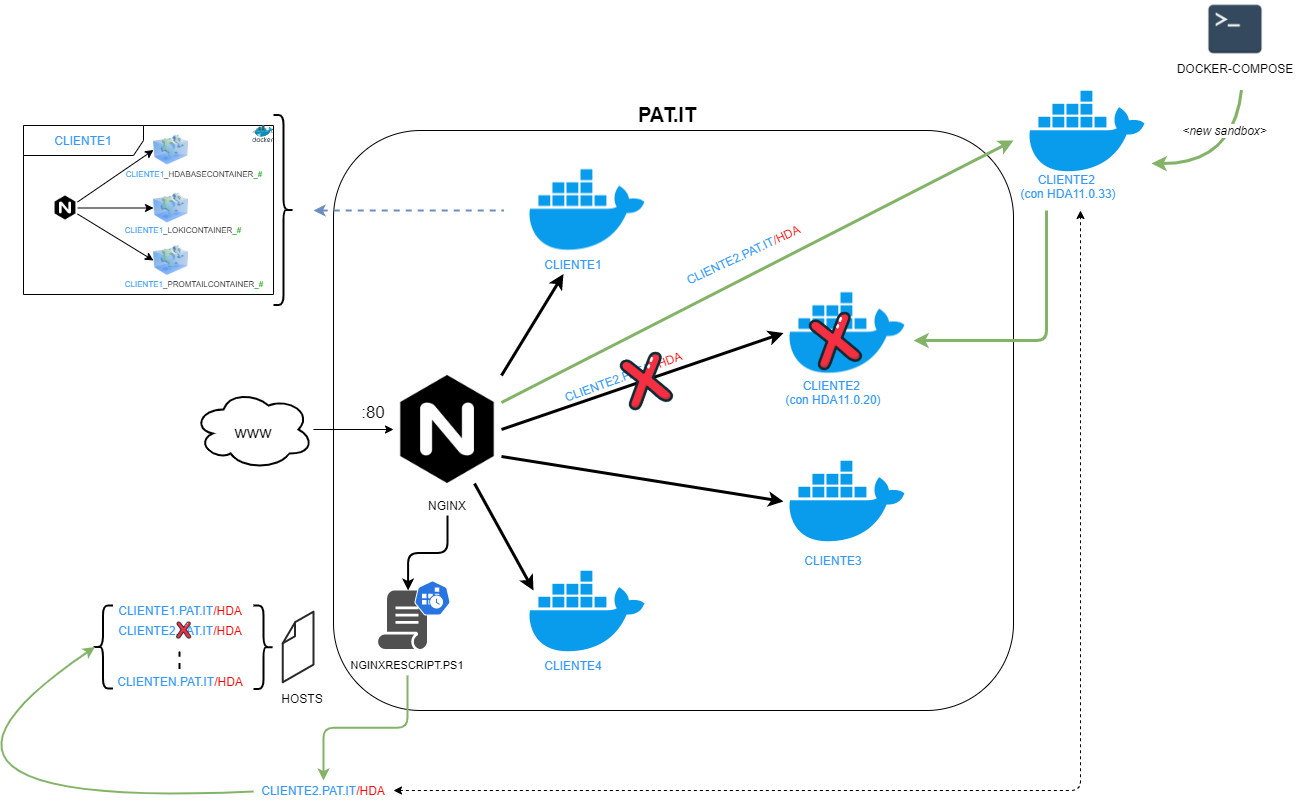
\includegraphics[width=1.0\columnwidth]{immagini/img/sandbox_nginx} 
    \caption{Rappresentazione grafica circa la gestione runtime delle \textit{sandbox} applicative di HDA}
\end{figure}\\
\newpage
Quanto sopra rappresentato, può essere facilmente riassunto nei seguenti passi:
\begin{enumerate}
	\item Arrivo della richiesta HTTP esterna (ex: cliente1.pat.it) all'NGINX dell'\textbf{host \textit{PAT.IT}};
	\item Il sistema operativo dell'host \textit{PAT.IT} controlla se l'FQDN della richiesta è presente all'interno del suo \textbf{file host};
	\item Il webserver NGINX controlla se l'entry "cliente1.pat.it" è presente nel suo \textbf{config file} (nginx.conf) e, se presente, provvede ad \textbf{inoltrare la richiesta} alla relativa \textit{sandbox};
	\item La richiesta HTTP \textbf{arriva al webserver NGINX interno} alla relativa \textit{sandbox} avente il nome uguale al prefisso della richiesta HTTP (ex: cliente1);
    	\item Il webserver NGINX interno alla \textit{sandbox} applicativa \textbf{inoltra la richiesta} HTTP al container "\textbf{hdabasecontainer}", permettendo quindi agli utenti dell'azienda "cliente1" il \textbf{totale accesso all'istanza di HDA};
	\item Eventuali programmi esterni di monitoring in real-time (quali, ad esempio, Grafana) possono ora essere collegati alla \textit{sandbox} applicativa semplicemente digitando nel relativo config-file (ex in Grafana: grafana.conf) l'\textbf{FQDN della relativa \textit{sandbox} da monitorare} (ex: cliente1.pat.it). Sarà compito del relativo NGINX interno alla \textit{sandbox} gestire e dirottare (tramite proprio file di configurazione nginx.conf) ai relativi container le richieste del programma di monitoring.
\end{enumerate}

\subsection{Aggiornamento di HDA nella sandbox applicativa}
Come precedentemente accennato in questo documento, e come rappresentato sempre nell'immagine 6.1, risulta facilmente intuibile la fattibilità di un eventuale aggiornamento di una relativa \textit{sandbox} applicativa. Per effettuare infatti un aggiornamento alla \textit{sandbox} applicativa di HDA, sarà sufficiente eseguire i seguenti passi:
\begin{enumerate}
	\item \textbf{Eliminazione} della \textit{sandbox} applicativa contenente la versione legacy di HDA;
	\item \textbf{Creazione} delle nuove immagini dei nuovi container della futura nuova \textit{sandbox} applicativa di HDA tramite batch-file \textbf{HDA\_sandbox\_builder.bat};
	\item Effettuare la \textbf{migrazione manuale} di eventuali \textit{overrides} o \textit{extensions} contenuti nella cartella App\_Data nel relativo volume-mapping nell'host ("hdashared");
	\item \textbf{Avviare}, tramite comando Docker Compose, la nuova \textit{sandbox} di HDA con il \textbf{nome uguale} alla \textit{sandbox} appena sostituita.
\end{enumerate}

Facendo questo, in maniera del tutto automatica, gli utenti accederanno così alla nuova istanza di HDA aggiornata.\\

Grazie al risolutore DNS interno a Docker ed al suo load-balancing automatico, nel caso di necessità di aggiornamento di \textbf{molteplici container} all'interno della \textit{sandbox} applicativa di HDA, si potrà aggiornare relativamente la versione di HDA in ogni container \textbf{senza generare alcun downtime} al cliente, semplicemente aggiornando \textbf{un container alla volta}, per permettere quindi al load-balancer di Docker di poter inoltrare tutte le richieste HTTP ad almeno un container attivo e funzionante di HDA. Il meccanismo di aggiornamento di multipli container all'interno di una singola \textit{sandbox} applicativa non era nei requisiti di questo stage né è stato in alcun modo testato dallo stagista durante tutto il periodo di stage. Questa possibilità di aggiornamento e di load-balancing dei container di HDA è stata sviluppata a livello completamente teorico dal sottoscritto e dal proprio tutor Ruggero Maffei con il preziosissimo aiuto del Sig. Adriano Trevisan.

\section{Analisi NginxREScript.ps1}
Nel caso in cui il lancio o rimozione di \textit{sandbox} applicative 
%**************************************************************             % Product Design Freeze e SOP
% !TEX encoding = UTF-8
% !TEX TS-program = pdflatex
% !TEX root = ../tesi.tex

%**************************************************************
\chapter{Conclusioni}
\label{cap:conclusioni}
\intro{Breve introduzione al capitolo}\\
Il presente capitolo finale vuole esporre una panoramica generale sul raggiungimento generale degli obiettivi dello stage curricolare, valutando le conoscenze acquisite dallo stagista e la qualità generale dell'esperienza di stage effettuata all'interno dell'Azienda.
\section{Raggiungimento degli obiettivi}
Come riportato nel capitolo 2.2, causa mole di lavoro troppo impegnativa in rapporto al tempo già rilevato ad inizio del percorso di stage, sotto completo suggerimento del tutor aziendale Sig. Maffei Ruggero, è stato consigliato al candidato di \textbf{concentrarsi esclusivamente sulla creazione di una immagine \textit{Dockerizzata} del solo prodotto HDA con le relative dipendenze}, come descritto nell'apposito capitolo prima citato.
Avendo l'Azienda stessa modificato già ad inizio stage la lista degli obiettivi obbligatori e desiderabili che il candidato avrebbe dovuto portare a termine, lo stagista è riuscito a portare a termine ed a soddisfare \textbf{tutti} gli obiettivi ed i requisiti con una settimana d'anticipo rispettivamente alla tabella oraria, \textbf{ad eccezione} del requisito che richiedeva la creazione di un container per l'esecuzione degli \textbf{unit test} automatici delle immagini create. La tabella sottostante rappresenta, graficamente, gli obiettivi e requisiti con il relativo stato di raggiungimento (\textbf{R}) o non raggiungimento (\textbf{NR}):
\newpage
\begin{center}
\begin{tabular}{|m{25em} | m{2,1cm} | m {1cm}|} 
 \hline
 \textbf{Descrizione requisito} & \textbf{Quantitativo orario (h)} & \textbf{Stato}\\ [0.5ex] 
 \hline\hline
 Introduzione al tema Container vs Virtual machine: differenze tra le due tecnologie e
illustrazione dei vantaggi derivanti dall'adozione dei Container & 40 & R\\ 
 \hline
 Docker ed estensioni (Docker, Compose e Swarm, Kubernetes) e relative API di
automation: analisi delle componenti dell'ecosistema e delle opportunità di utilizzarle
ai fini progettuali & 40 & R\\
 \hline
 Approfondimento sull'architettura su due casi studi da containerizzare: declinazione
della soluzione tecnologica identificata ai punti precedenti su due applicazioni PAT & 120 & R\\
 \hline
 Creazione dei container ed automatizzazione del processo di building: realizzazione
del processo di creazione delle immagini ed automazione dello stesso & 80 & R\\
 \hline
 Utilizzo di un container per verifica dell'esecuzione degli unit test: avvio delle
immagini per effettuazione degli unit test in automatico & 40 & NR\\ [1ex] 
 \hline
 \textbf{TOTALE} & \textbf{320} & \textbf{4/5}\\
 \hline
\end{tabular}
\end{center}
La settimana avanzata è stata usata dal candidato per la \textbf{scrittura di tutta la documentazione di supporto} interna all'Azienda, per permettere ai lavoratori di capire ed ampliare in futuro quanto sviluppato durante tutta l'esperienza di stage. La documentazione redatta è stata inserita nell'apposita sezione \textbf{OneNote} dell'Azienda assieme a tutta la documentazione interna dei loro prodotti.

%**************************************************************
\section{Conoscenze acquisite}
Le conoscenze conseguite a seguito dell'esperienza di stage sono state molteplici, in primis tra tutte la \textbf{tecnologia} che ho implementato. L'aver studiato in maniera approfondita la tecnologia Docker mi ha permesso di rendermi conto dell'esistenza di una tecnologia\textbf{ completamente alternativa}, e per molti aspetti altrettanto valida, alle classiche \textbf{architetture a macchine virtuali}, con conseguente mia possibilità di ulteriore approfondimento e studio individuale futuro nell'ottica di poter proporre, alle future aziende con le quali collaborerò, delle \textbf{soluzioni architetturali non più basate solo ed esclusivamente sulle virtual machine}.\\
A livello umano, ho trovato \textbf{persone estremamente preparate e professionali} con cui sono tutt'ora in contatto. Queste persone hanno contribuito alla mia \textbf{crescita interiore} facendomi rendere conto che, in un clima di reciproca fiducia e collaborazione, qualsiasi progetto, se ben supportato da colleghi attenti e preparati, potrà essere sviluppato con successo senza un rischio elevato di fallimento immediato ed a lungo termine. Avendo lavorato in un team così dinamico, ho inoltre \textbf{rivisto la mia metodologia di lavoro}, tipicamente molto autonoma, nell'ottica di una mia sempre più \textbf{aperta visione ad eventuali osservazioni ed insegnamenti} dettati da dipendenti con molta più preparazione ed esperienza alle loro spalle rispetto al sottoscritto. Questi insegnamenti rientreranno senz'altro nel mio \textbf{bagaglio culturale}, nella speranza di \textit{saperli} e \textit{poterli} attuare in ulteriori esperienze lavorative.

%**************************************************************
\section{Valutazione personale}
La mia personale opinione su questa esperienza di stage non può che essere \textbf{assolutamente positiva}. Ho avuto l'opportunità di lavorare a contatto con un team \textbf{altamente qualificato}, e di conoscere persone molto competenti nel loro ambito che spero continuino a far parte della mia rete di amicizie. \\
L'aver fatto questa esperienza di stage mi ha, inoltre, permesso di apprendere com'è \textbf{organizzata internamente} un'azienda informatica di medie dimensioni. L'avermi dovuto rapportare con diverse persone di grado differente ha fatto sì che abbia potuto\textbf{ mettere alla prova la mia capacità di relazionarmi con le persone}, diversificando, naturalmente, la mia metodologia di interlocuzione a seconda del ruolo del componente dell'Azienda con cui mi stavo confrontando.\\
Sempre grazie a questa esperienza di tirocinio, ho imparato a \textbf{gestire il mio tempo} in maniera nettamente \textbf{migliore} rispetto a tutto il percorso universitario fatto. Il dovermi rapportare con scadenze settimanali, riunioni di avanzamento e vincoli, obbligatori e non, hanno contribuito a sviluppare in me una \textbf{migliore capacità di gestione temporale}, facendomi imparare, in primis, che il tempo utilizzato per lo studio di una particolare tecnologia è forse la \textbf{parte più importante di un progetto stesso}, e che quindi va eseguita senza alcuna fretta o pregiudizio.







             % Conclusioni
\appendix                               
% !TEX encoding = UTF-8
% !TEX TS-program = pdflatex
% !TEX root = ../tesi.tex

%**************************************************************


             % Appendice A

%**************************************************************
% Materiale finale
%**************************************************************
\backmatter
\printglossaries
% !TEX encoding = UTF-8
% !TEX TS-program = pdflatex
% !TEX root = ../tesi.tex

%**************************************************************
% Bibliografia
%**************************************************************

\cleardoublepage
\chapter{Bibliografia}

\nocite{*}
% Stampa i riferimenti bibliografici
\printbibliography[heading=subbibliography,title={Riferimenti bibliografici},type=book]

% Stampa i siti web consultati
\printbibliography[heading=subbibliography,title={Siti web consultati},type=online]


\end{document}
